%% This is an example first chapter.  You should put chapter/appendix that you
%% write into a separate file, and add a line \include{yourfilename} to
%% main.tex, where `yourfilename.tex' is the name of the chapter/appendix file.
%% You can process specific files by typing their names in at the 
%% \files=
%% prompt when you run the file main.tex through LaTeX.

\begingroup%
\makeatletter%
\cleardoublepage%
\let\newpage\relax%
\let\clearpage\relax%
\vspace*{\fill}%
\vspace*{\dimexpr-50\p@-\baselineskip}% Remove the initial
%% -default- 50pt gap (plus 1 line) 
\chapter[Supporting information for Chapter 3]{{\setlength{\huge} Supporting information for}\\ \autoref{chap3}: LOBSTAHS: \\An Adduct-Based\\Lipidomics Strategy for \\Discovery and Identification of Oxidative Stress \\Biomarkers}
\label{AppD}
\let\thefootnote\relax\footnote{{\setlength{\parindent}{0pt}This supporting information was originally published in conjunction with:\\\\Collins, J. R., B. R. Edwards, Helen F. Fredricks, and B. A. S. Van Mooy. 2016. LOBSTAHS: An adduct-based lipidomics strategy for discovery and identification of oxidative stress biomarkers. \emph{Analytical Chemistry} \emph{88}:7154-7162; doi:\href{http://dx.doi.org/10.1021/acs.analchem.6b01260}{10.1021/acs.analchem.6b01260}\\\\\copyright 2016 American Chemical Society}}
\vspace*{\fill}%
\endgroup%

\clearpage

\section{Supplementary Methodological Details Not Described in the Text}
\label{sec:Supplementary Methodological Details Not Described in the Text}

\subsection{Conversion of .raw Data Files to .mzXML Format}

After acquiring data from the mass spectrometer, we employed a short, custom R script (\href{https://github.com/vanmooylipidomics/LipidomicsToolbox/blob/master/Exactive_full_scan_process_ms1+.r}{Exactive\_full\_scan\_process\_ms1+.R}) to automate three functions of the msConvert (Kessner et al., 2008) command-line tool. The script first converts all Thermo .raw files in a given dataset to the open-source .mzXML format, which is used by many chromatographic alignment and peak picking applications. It then converts the profile-mode mass spectral data in each file to a series of centroids. Finally, the script automates the extraction of the positive and negative ion mode full scan events from each sample into separate files. In the Exactive instrument configuration described in the text, the full scan events from the two ion modes appeared in each data file as the first and third scan events at each time point, respectively. (The second and fourth scan events at each time point were the positive and negative mode AIF scans.) The extraction and separation of scans from the two ion modes was necessary to accomplish subsequent analysis using the pipeline. In our analysis of the \emph{P. tricornutum} dataset, we omitted from this step two blanks and data from two samples collected at the 4 h timepoint (one of two replicates from each of the 0 $\mu$M and 150 $\mu$M H\textsubscript{2}O\textsubscript{2} treatments) because of an unexpected shift in chromatography that rendered the data incompatible with our analysis.

\subsection{Sample Injection, Chromatography and ESI Source Settings}
\label{ssec:Sample Injection, Chromatography and ESI Source Settings}

20 $\mu$L injections of sample were made onto a C8 Xbridge HPLC column (particle size 5 $\mu$m, length 150 mm, width 2.1 mm; Waters Corp., Milford, MA, USA). Eluent A consisted of water with 1\% 1M ammonium acetate and 0.1\% acetic acid. Eluent B consisted of 70\% acetonitrile, 30\% isopropanol with 1\% 1M ammonium acetate and 0.1\% acetic acid. Gradient elution was performed with the following program (total run time 30 min) at a constant flow rate of 0.4 mL min\textsuperscript{-1}: 45\% A for 1 min to 35\% A at 4 min, then from 25\% A to 11\% A at 12 min, then to 1\% A at 15 min with an isocratic hold until 25 min, and finally back to 45\% A for 5 min column equilibration. ESI source settings were: Spray voltage, 4.5kV (+), 3.0 kV (-); capillary temperature, 150$^{\circ}$C; sheath gas and auxiliary gas, both 21 (arbitrary units); heated ESI probe temperature, 350$^{\circ}$C.

\subsection{Mass Spectrometer Acquisition Settings}

Mass data were collected on a ThermoFisher Exactive Plus Orbitrap instrument in full scan (FS) and all-ion-fragmentation modes (AIF) while alternating between positive and negative ion modes. A scan range of 150-1500 \emph{m/z} was used for all modes in sequence (FT MS positive full scan, FT MS positive AIF, FT MS negative full scan, and FT MS negative AIF, respectively). The S-lens RF level was set to 85.00. Mass resolution was set to the maximum possible value of 140,000 (FWHM at \emph{m/z} 200) for both FS and AIF. This mass resolution setting corresponded to an observed resolution of 75,100 at the \emph{m/z} (875.5505) of our internal standard, DNP-PE. The observed resolution at \emph{m/z} 1269.0952, that of the compound in the screened dataset with the highest molecular weight (TAG 76.6 +4O), was 41,100. Using these settings, we obtained between 8 and 14 MS scans across a typical peak.

\subsection{Procedures Used for Weekly and Real-Time Calibration of the Exactive}

The mass spectrometer was calibrated weekly in both positive and negative ion modes by infusing calibration mixes available from ThermoFisher Scientific. Low-level eluent contaminants were also utilized as lock masses, providing real-time recalibration; C16:0 (255.23295) and C18:0 (283.26425) fatty acids were used in negative ion mode, while a polysiloxane (536.16537) and phthalate (391.28429) were used in positive ion mode. At least one of the lock masses was found during each positive and negative full scan event.

\subsection{Script for Pre-Processing Data in xcms and CAMERA}

We implemented xcms and CAMERA using the script \href{https://github.com/vanmooylipidomics/LipidomicsToolbox/blob/master/prepOrbidata.R}{prepOrbidata.R}, a version of which is available under the MIT License at \texttt{\href{https://github.com/vanmooylipidomics/LipidomicsToolbox}{https://github.com/vanmooylipidomics/LipidomicsT\\oolbox}}. Users can modify the script as necessary. We used the R package IPO to optimize settings for xcms and CAMERA, obtaining the parameter values given in \autoref{table:adn5}. We used these parameter values to obtain the results presented in the text.

\subsection{Determination of Retention Time Window Data}

The retention time (RT) window data in \autoref{table:adn4} were obtained primarily from authentic standards for representative compounds of each parent lipid class under the chromatographic conditions described in the text. Observations of various lipids in environmental samples allowed us to consider additional species. While LOBSTAHS applies the retention time data contained in \autoref{table:adn4} as a default, detailed instructions and an example data table are included in the onboard documentation for use with retention time data for other chromatographic methods. As for the adduct ion hierarchy data, retention time data for ox-IPL are inherited from the unoxidized parent molecule. By default, LOBSTAHS expands the retention time window for each lipid class by 20\% of its given width to account for (1) shifts in retention time that may occur during chromatographic alignment with xcms and (2) slight variations in retention time that distinguish the different positional (i.e., regio-) isomers of the same parent lipid (Yang et al., 2009; G\"{o}bel and Feussner, 2009). This window can be narrowed or expanded with user input.

\subsection{Analysis of Positive Ionization Mode \emph{P. tricornutum} Data Using xcms, CAMERA, and LOBSTAHS}

To examine the effect of oxidative stress on the \emph{P. tricornutum} lipidome, we applied the LOBSTAHS workflow (\autoref{fig:c3n1}) to a dataset assembled from only positive mode data files. We confined our analysis to the positive mode data because intact polar lipids (IPL), the primary targets of both reactive oxygen species (ROS) and lipoxygenase-mediated enzymatic transformations induced by H\textsubscript{2}O\textsubscript{2}, are most amenable to analysis in positive ion mode. The specific workflow and parameter values we applied to the dataset in xcms, CAMERA, and LOBTAHS are given in \autoref{table:adn5}. We elected to apply all three optional filters to the data in LOBSTAHS.

\subsection{Choice of Matching Tolerance}

To account for variability in performance expected from natural samples, we used a 2.5 ppm mass uncertainty tolerance when matching against the databases. This tolerance was one order of magnitude more conservative than the 0.22 ppm mass uncertainty we observed with authentic standards (\autoref{table:c3n1} and \autoref{table:adn6}), yet considerably more restrictive than the various default standards used for matching in other recently introduced metabolomics applications (Gaquerel et al., 2013; Wolf et al., 2010). When combined with HPLC separation and the high mass resolution of the Exactive, the 2.5 ppm tolerance still allowed us to assign distinct identities to isobaric masses.

\subsection{Statistical Analysis and Visualization of the \emph{P. tricornutum} Lipidome }

The LOBSTAHS workflow is designed to facilitate examination of relative changes in the abundances of lipids in a given dataset, not to enable absolute quantification of specific analytes or direct comparisons between datasets. With this in mind, the annotated output from LOBSTAHS was used to calculate the relative abundances of \emph{P. tricornutum} lipidome constituents present in the 0 and 150 $\mu$M H\textsubscript{2}O\textsubscript{2} treatments at 24 h. The analysis was performed as follows:

First, using the script \href{https://github.com/jamesrco/LipidomicsDataViz/blob/master/LOBSTAHS/PtH\textsubscript{2}O\textsubscript{2}_mz-rt_plots.R}{PtH\textsubscript{2}O\textsubscript{2}\_mz-rt\_plots.R}, we extracted from the processed dataset a subset of ``high confidence'' assignments to be used in all subsequent analyses (i.e., assignments annotated with codes C1 or C2a and having no identified structural isomers or isobars; \autoref{fig:c3n2}a and symbols with darkest tones in \autoref{fig:adn2}-\autoref{fig:adn10}). The remaining putative assignments we classified as ``moderate confidence,'' indicating that the underlying features satisfied the hierarchy rules fundamentally yet imperfectly (symbols with lighter tones in \autoref{fig:adn2}-\autoref{fig:adn10}). The peak areas of the high confidence assignments were normalized to data for an internal standard (DNP-PE). We then further restricted our analysis to only those compounds still present in two or more samples. (\href{https://github.com/jamesrco/LipidomicsDataViz/blob/master/LOBSTAHS/PtH\textsubscript{2}O\textsubscript{2}_mz-rt_plots.R}{PtH\textsubscript{2}O\textsubscript{2}\_mz-rt\_plots.R} and the other scripts referenced in \autoref{AppD} are available from \url{https://github.com/jamesrco/LipidomicsDataViz)}

Using the script \href{https://github.com/jamesrco/LipidomicsDataViz/blob/master/LOBSTAHS/PtH\textsubscript{2}O\textsubscript{2}_heatmap_sigclust.R}{PtH\textsubscript{2}O\textsubscript{2}\_heatmap\_sigclust.R}, peak areas of the remaining assignments were then scaled using a level approach according to van den Berg et al. (2006). Each peak area, ${x_i}$, was divided by the average peak area of that compound across the dataset, ${x_{avg}}$, to obtain a normalized peak area, ${\tilde x_i}$:
\begin{equation} \label{eq:adn1}
{\tilde x_i} = \frac{{{x_i}}}{{{x_{avg}}}}
\end{equation}
Values of ${\tilde x_i}$ were then used in the steps described below to represent the relative abundances of the compounds present in each sample.

When the same compound appeared in duplicates of the same experimental treatment, values of ${\tilde x_i}$ were averaged. Since subsequent statistical analysis required log\textsubscript{2} transformation of the data and many hierarchical clustering functions cannot use values of 0 or ``NA'' as inputs, all values of ${\tilde x_i}$ equal to 0 were replaced with 10\textsuperscript{-6}.

The heatmaps and dendrogram in \autoref{fig:c3n3} and \autoref{fig:adn11} were then generated from this subset of relative abundances using the R packages gplots (Warnes et al., 2016) and clustsig (Whitaker and Christman, 2014). Similarity profile analysis (Clarke et al., 2008) was then used to cluster the molecular species in the subset according to their degree of covariation. The groups of lipidome components identified by this similarity profile analysis are presented in \autoref{table:adn8}. Following this analysis, the heatmaps in \autoref{fig:c3n3} and \autoref{fig:adn11} was reordered and the dendrogram was rotated such that the order of compounds in both figures is from most upregulated in the 150 $\mu$M H\textsubscript{2}O\textsubscript{2} treatment to most downregulated. The groups from the similarity profile analysis (\autoref{table:adn8}) were categorized by the general response of their components to H\textsubscript{2}O\textsubscript{2} treatment at 150 $\mu$M H\textsubscript{2}O\textsubscript{2}: 101 groups contained a total of 562 compounds more abundant in the 150 $\mu$M treatment (i.e., upregulated), 70 groups contained a total of 308 compounds less abundant in the 150 $\mu$M treatment (i.e., downregulated), and 11 groups together contained 26 components whose abundance was not significantly different between the two treatments (\emph{p} $\leq$ 0.01).

\clearpage

\section{Supplementary Figures}

\begin{figure}[!th]
\centering
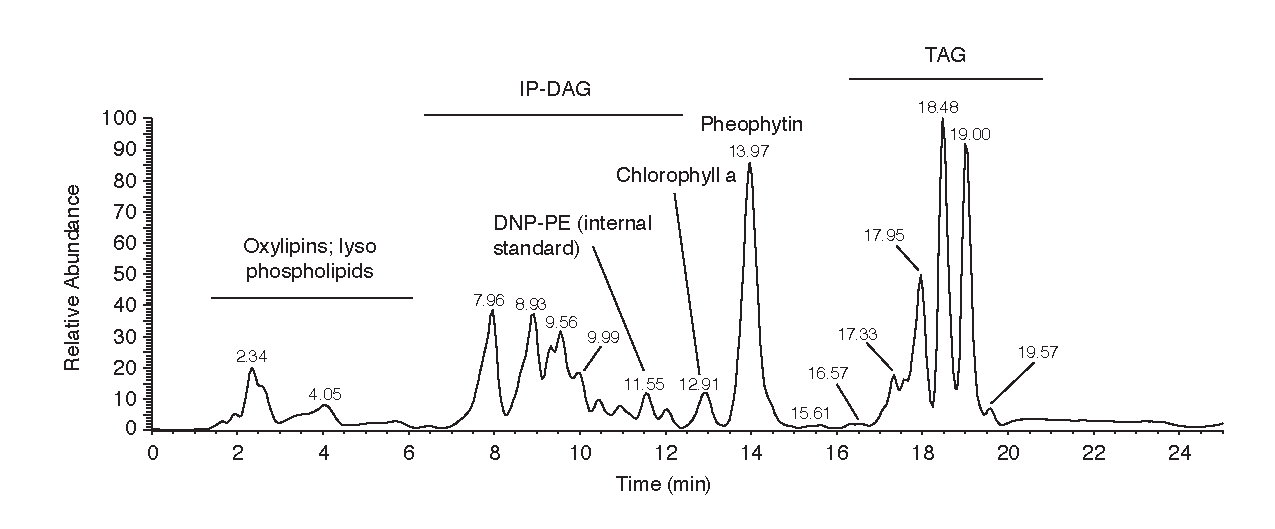
\includegraphics[width=1\textwidth]{Fig_D-1.pdf}
\captionsetup{font={footnotesize}}
\caption[Extracted ion chromatogram from a \emph{P. tricornutum} sample treated with 150 $\mu$M H\textsubscript{2}O\textsubscript{2}]{Extracted ion chromatogram (\emph{m/z} 500-1500; positive ion mode) from a \emph{P. tricornutum} sample treated with 150 $\mu$M H\textsubscript{2}O\textsubscript{2}. Spectra were acquired under the MS and HPLC conditions described in \autoref{ssec:Sample Injection, Chromatography and ESI Source Settings}. Text annotations show prominent identifiable features and retention time ranges of some different lipid classes.}
\label{fig:adn1}
\end{figure}

\clearpage

\begin{footnotesize}
\begin{singlespace}
{\setlength{\parindent}{0pt}
Following pages: Oxidized and intact species of nine classes of lipid identified in the \emph{P. tricornutum} dataset after 24 hours in (a) the control (0 $\mu$M H\textsubscript{2}O\textsubscript{2}) and (b) 150 $\mu$M H\textsubscript{2}O\textsubscript{2} treatments. \autoref{fig:adn2}, \autoref{fig:adn3}, \autoref{fig:adn4}, \autoref{fig:adn5}, \autoref{fig:adn6}, \autoref{fig:adn7}, \autoref{fig:adn8}, \autoref{fig:adn9}, and \autoref{fig:adn10} show species of, respectively, DGCC, DGDG, DGTS \& DGTA, MGDG, PC, PE, PG, SQDG, and TAG. Shading indicates the degree of confidence in the identification, while symbols indicate the degree of oxidation by addition of one or more oxygen atoms. Excluded are those compounds having an odd total number of acyl carbon atoms, according to the reasoning described in the text; this exclusion is an optional, user-electable LOBSTAHS screening feature. Where practical, a text annotation indicates the number of acyl carbon atoms and double bonds in each compound. Data are presented for a single experiment with two technical replicates.\\
\emph{\textsuperscript{a}} Darkest tones indicate high and moderate confidence IDs for which no structural isomers or isobars were detected; these are compounds annotated with codes ``C1,'' ``C2a,'' or ``C2b'' in the LOBSTAHS workflow illustrated in \autoref{fig:c3n1}.\\
\emph{\textsuperscript{b}} $\geq$ 1 structural isomer of an adduct of this compound is present in dataset (\autoref{fig:c3n1}, code C3f).\\
\emph{\textsuperscript{c}} Adduct ion of $\geq$ 1 other compound is an isobar of the dominant adduct of this compound; i.e., \emph{m/z} of the adducts are $\leq$ the 2 ppm match tolerance used in initial assignments (\autoref{fig:c3n1}, code C3c).\\
\emph{\textsuperscript{d}} $\geq$ 1 structural isomer and $\geq$ 1 competing assignment of second type both present.\\
\emph{\textsuperscript{e}} Compounds of which multiple regioisomers were identified in single sample, indicating possible oxidation of the same parent molecule at different structural positions.\\
\emph{\textsuperscript{f}} General direction of movement within \emph{m/z} versus RT plot for a given lipid class and oxidation state.
}
\end{singlespace}
\end{footnotesize}

\clearpage

\begin{figure}[!th]
\centering
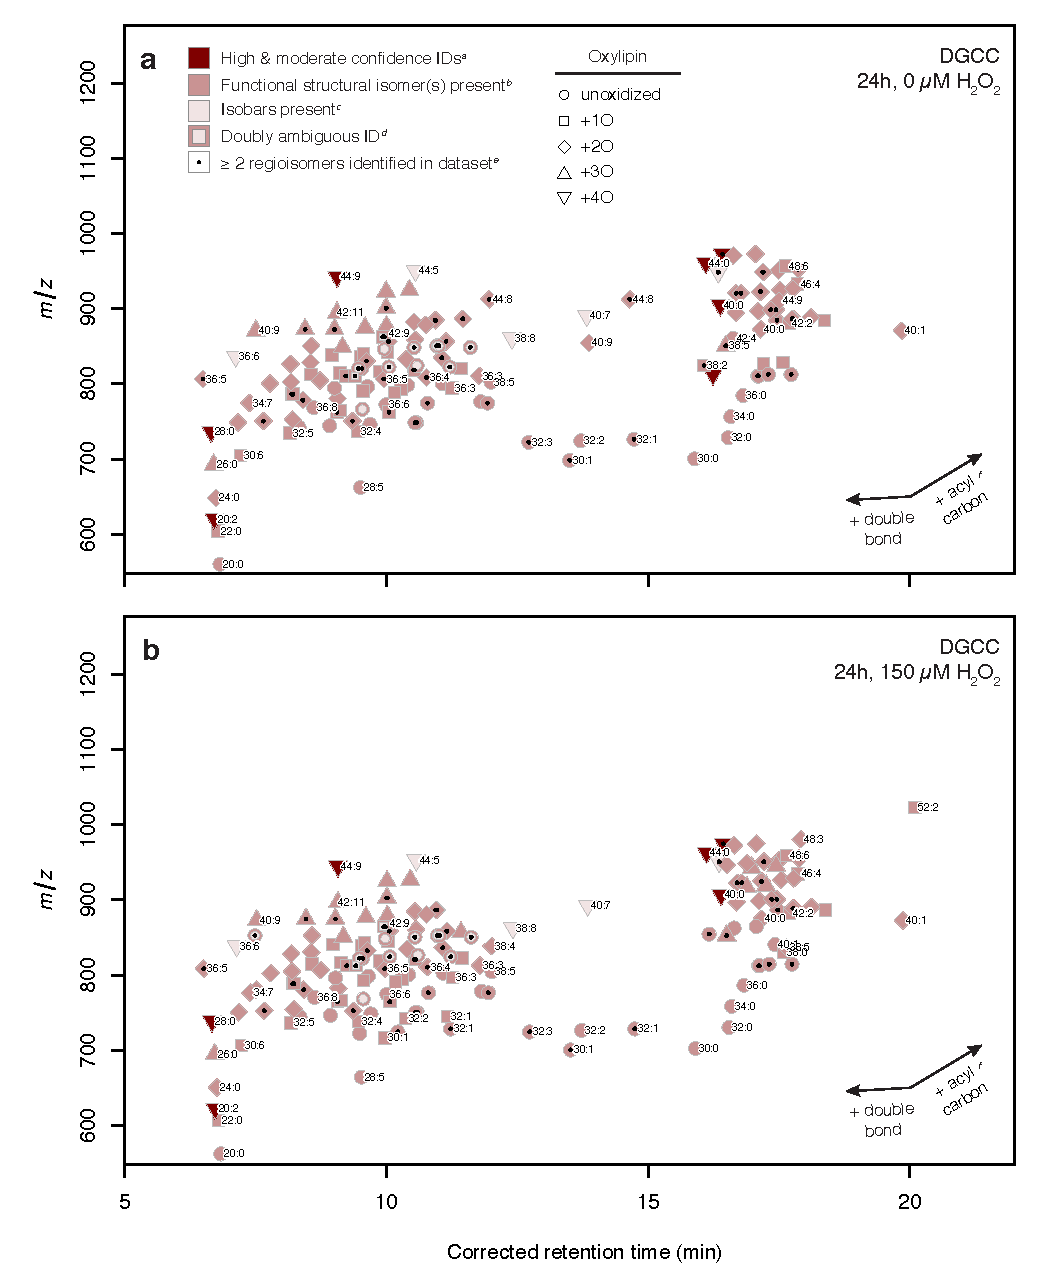
\includegraphics[width=1\textwidth]{Fig_D-2.pdf}
\captionsetup{font={footnotesize}}
\caption[Oxidized and intact species of DGCC identified in the \emph{P. tricornutum} dataset after 24 hours]{Oxidized and intact species of DGCC identified in the \emph{P. tricornutum} dataset after 24 hours.}
\label{fig:adn2}
\end{figure}

\clearpage

\begin{figure}[!th]
\centering
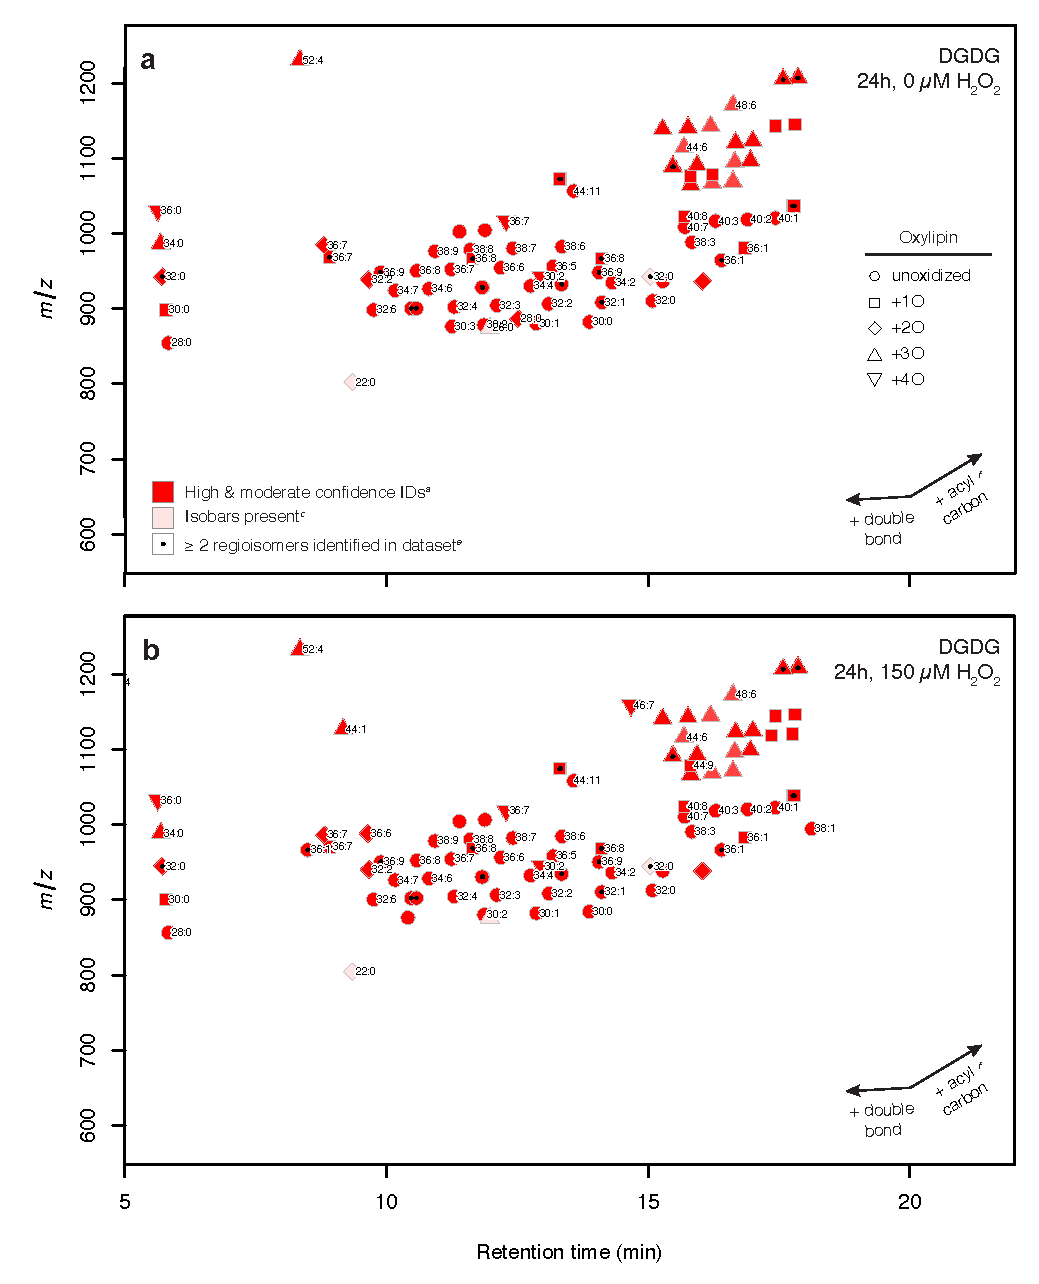
\includegraphics[width=1\textwidth]{Fig_D-3.pdf}
\captionsetup{font={footnotesize}}
\caption[Oxidized and intact species of DGDG identified in the \emph{P. tricornutum} dataset after 24 hours]{Oxidized and intact species of DGDG identified in the \emph{P. tricornutum} dataset after 24 hours.}
\label{fig:adn3}
\end{figure}

\clearpage

\begin{figure}[!th]
\centering
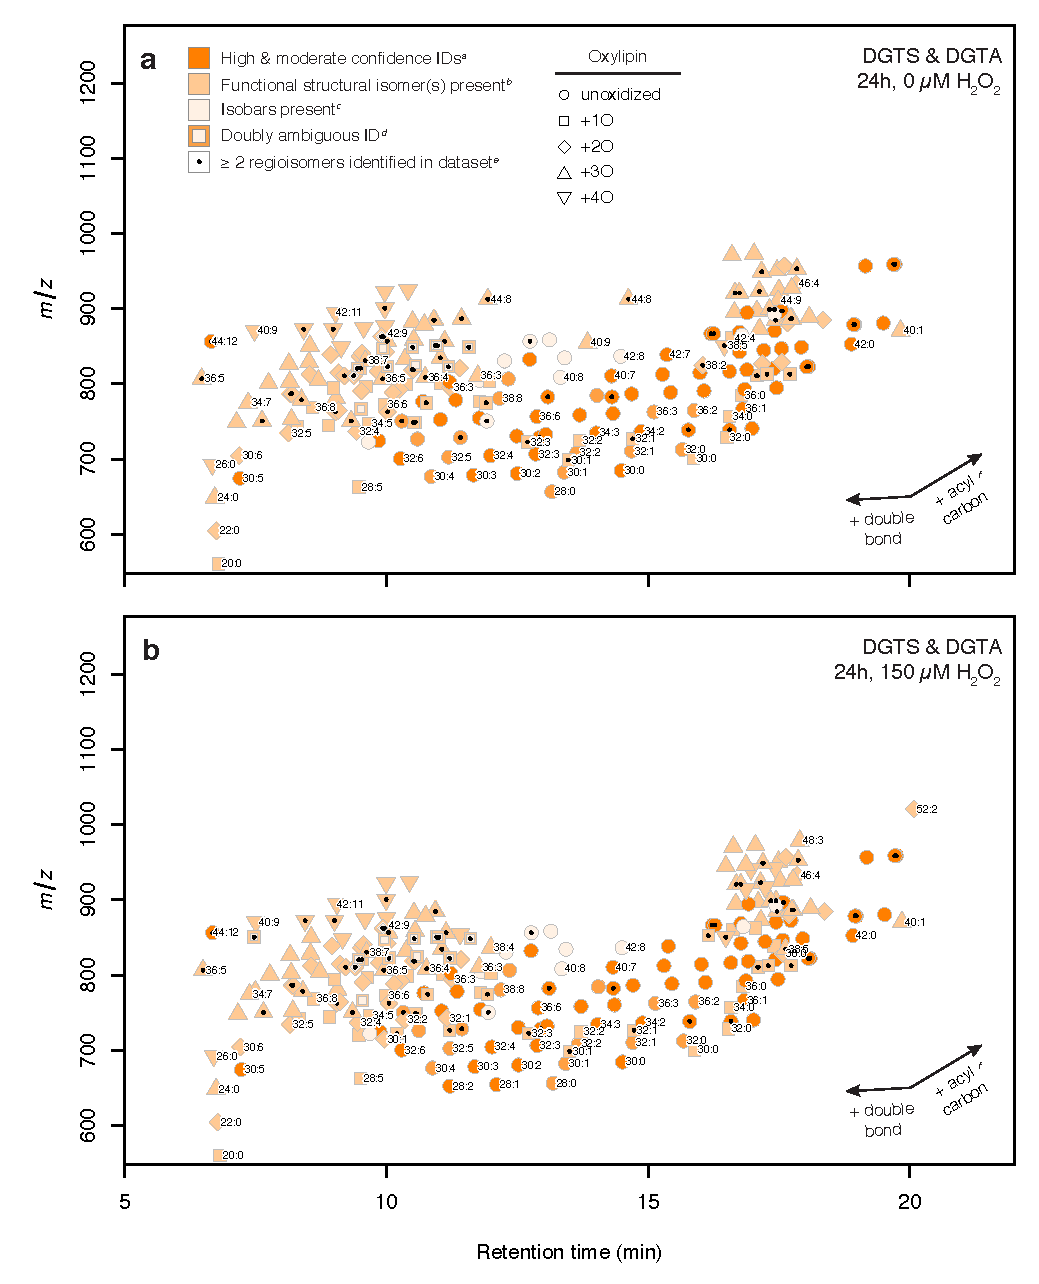
\includegraphics[width=1\textwidth]{Fig_D-4.pdf}
\captionsetup{font={footnotesize}}
\caption[Oxidized and intact species of DGTS \& DGTA identified in the \emph{P. tricornutum} dataset after 24 hours]{Oxidized and intact species of DGTS \& DGTA identified in the \emph{P. tricornutum} dataset after 24 hours.}
\label{fig:adn4}
\end{figure}

\clearpage

\begin{figure}[!th]
\centering
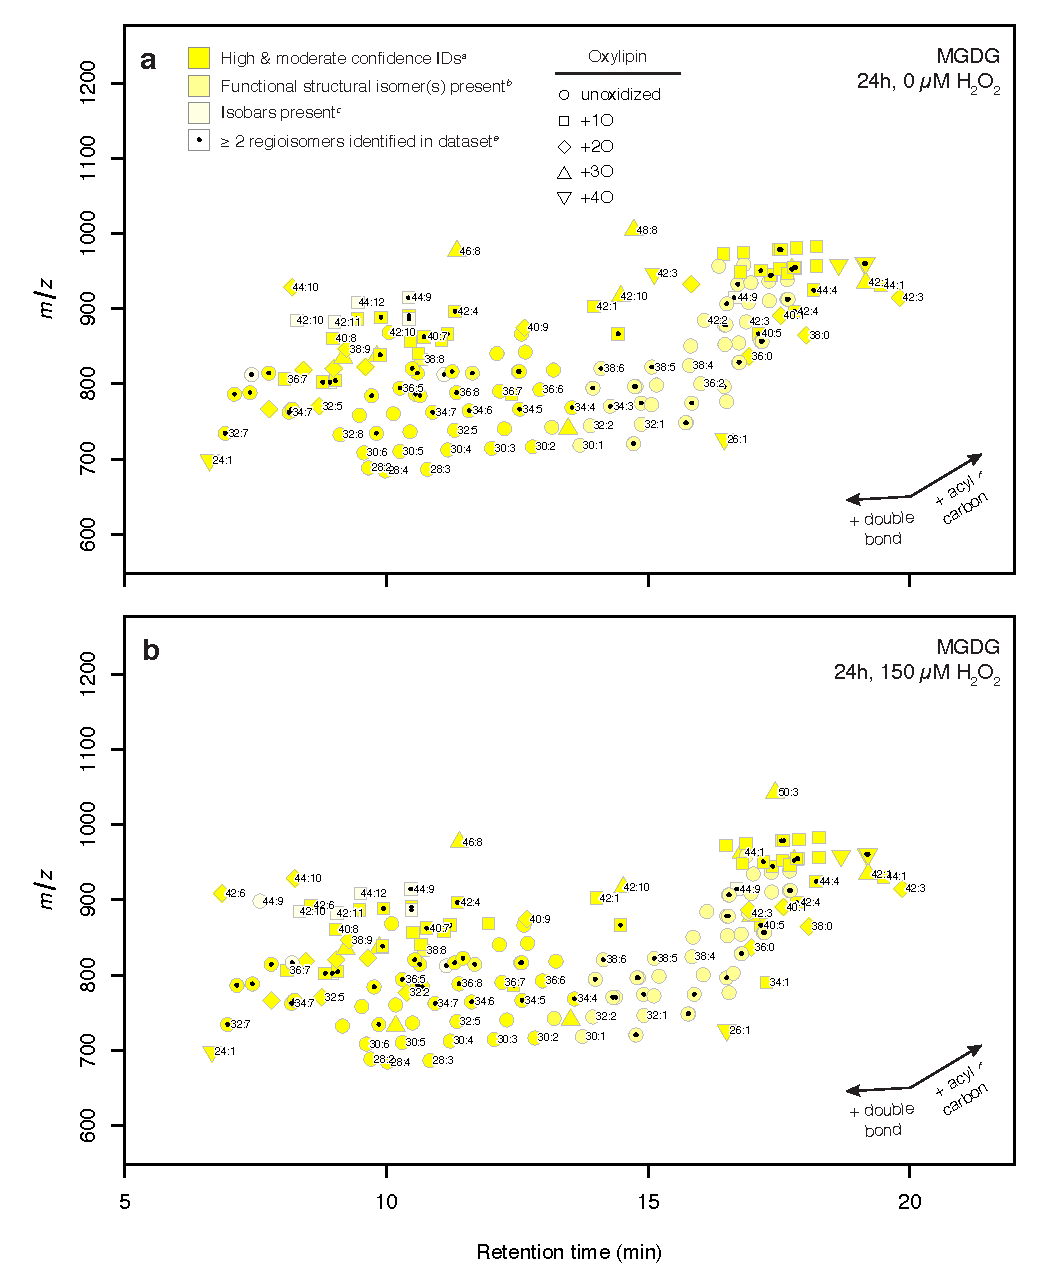
\includegraphics[width=1\textwidth]{Fig_D-5.pdf}
\captionsetup{font={footnotesize}}
\caption[Oxidized and intact species of MGDG identified in the \emph{P. tricornutum} dataset after 24 hours]{Oxidized and intact species of MGDG identified in the \emph{P. tricornutum} dataset after 24 hours.}
\label{fig:adn5}
\end{figure}

\clearpage

\begin{figure}[!th]
\centering
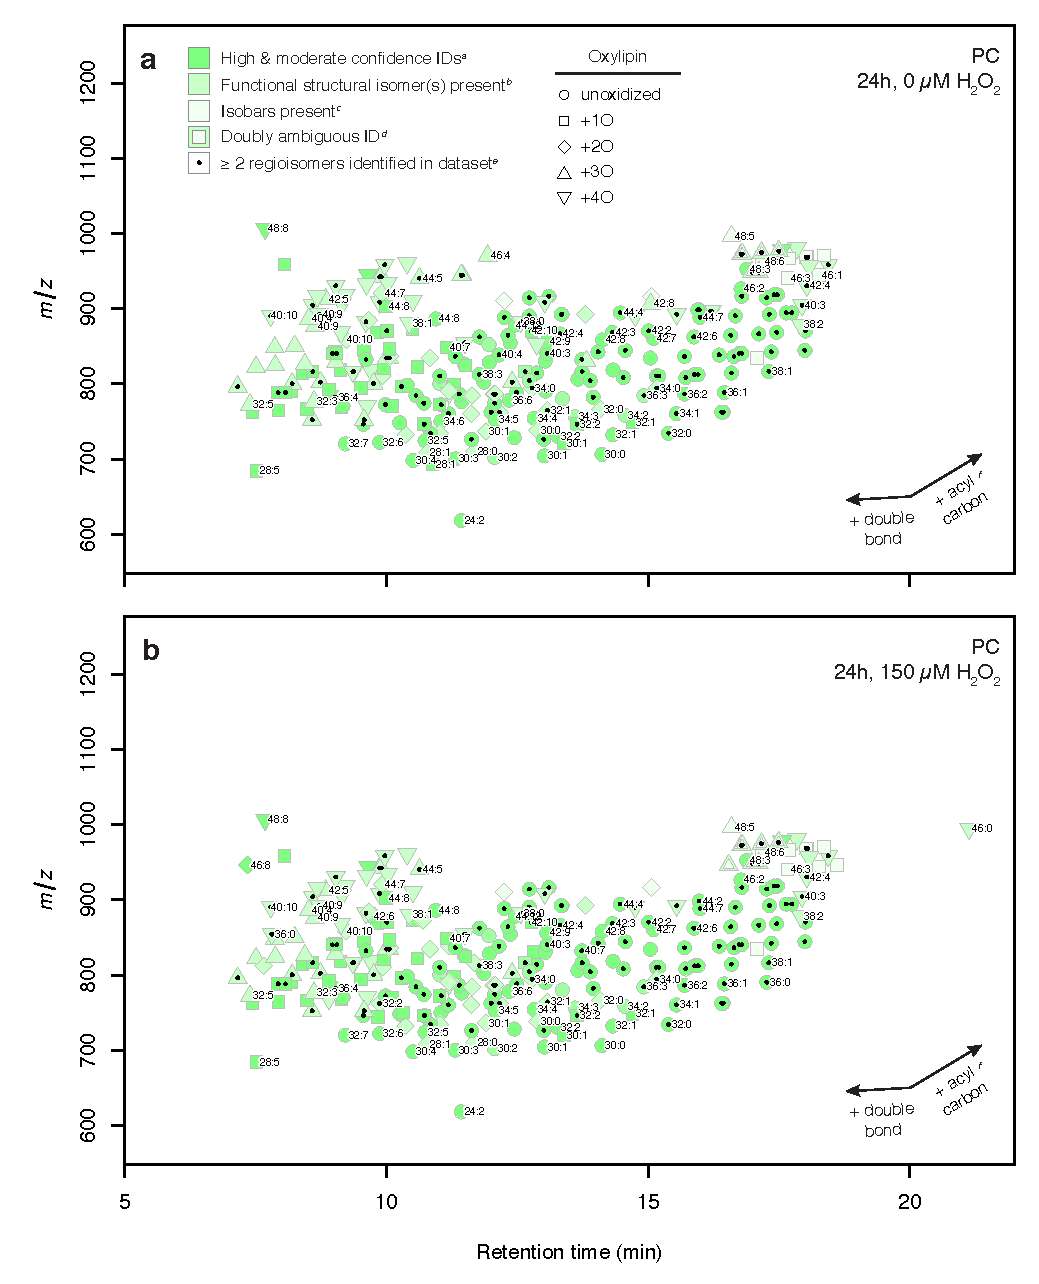
\includegraphics[width=1\textwidth]{Fig_D-6.pdf}
\captionsetup{font={footnotesize}}
\caption[Oxidized and intact species of PC identified in the \emph{P. tricornutum} dataset after 24 hours]{Oxidized and intact species of PC identified in the \emph{P. tricornutum} dataset after 24 hours.}
\label{fig:adn6}
\end{figure}

\clearpage

\begin{figure}[!th]
\centering
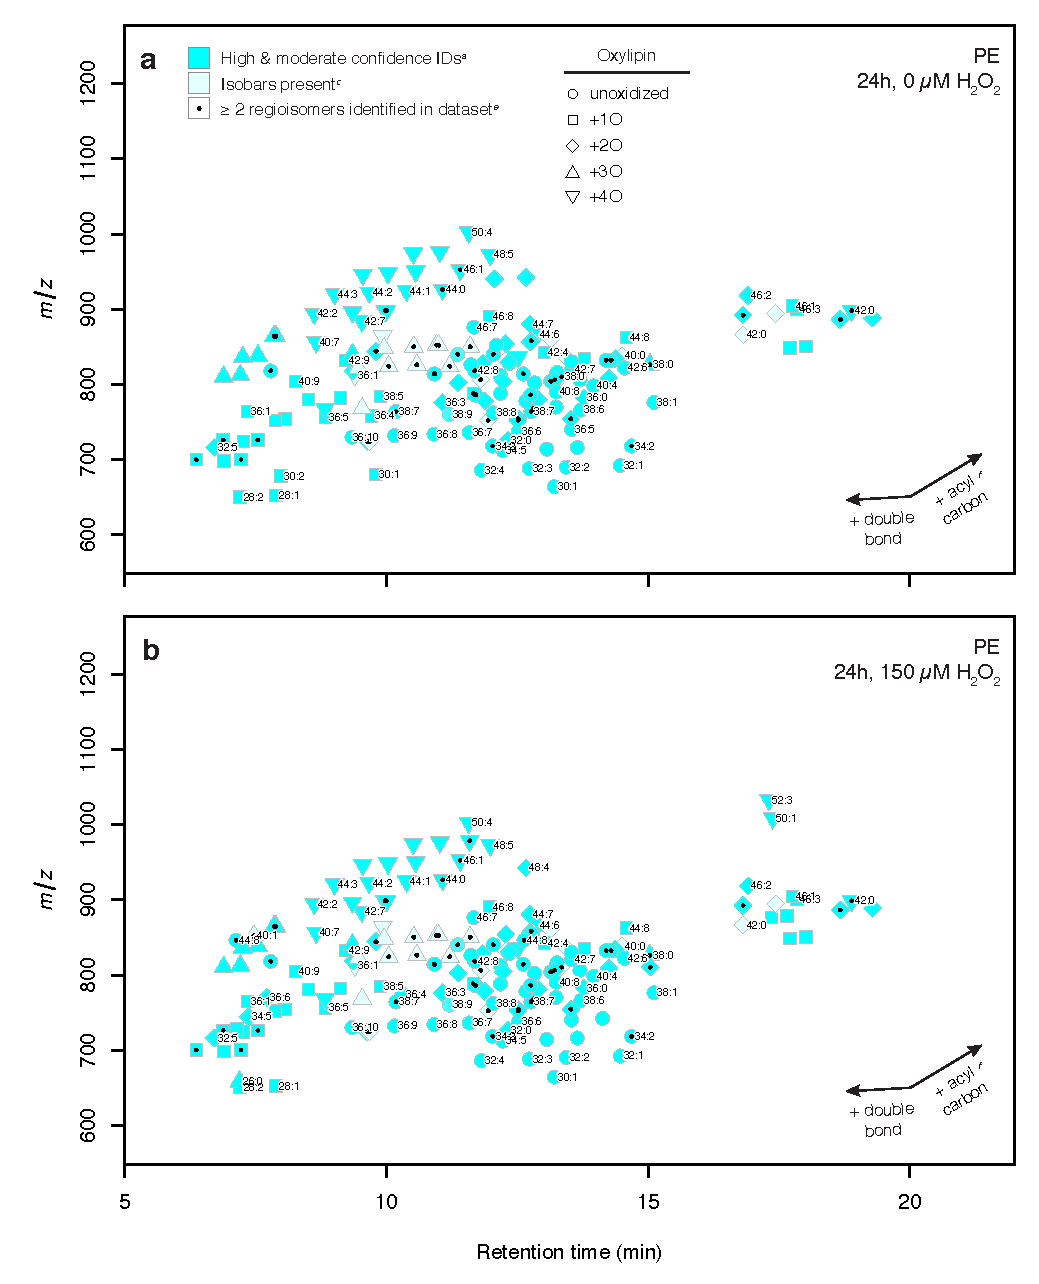
\includegraphics[width=1\textwidth]{Fig_D-7.pdf}
\captionsetup{font={footnotesize}}
\caption[Oxidized and intact species of PE identified in the \emph{P. tricornutum} dataset after 24 hours]{Oxidized and intact species of PE identified in the \emph{P. tricornutum} dataset after 24 hours.}
\label{fig:adn7}
\end{figure}

\clearpage

\begin{figure}[!th]
\centering
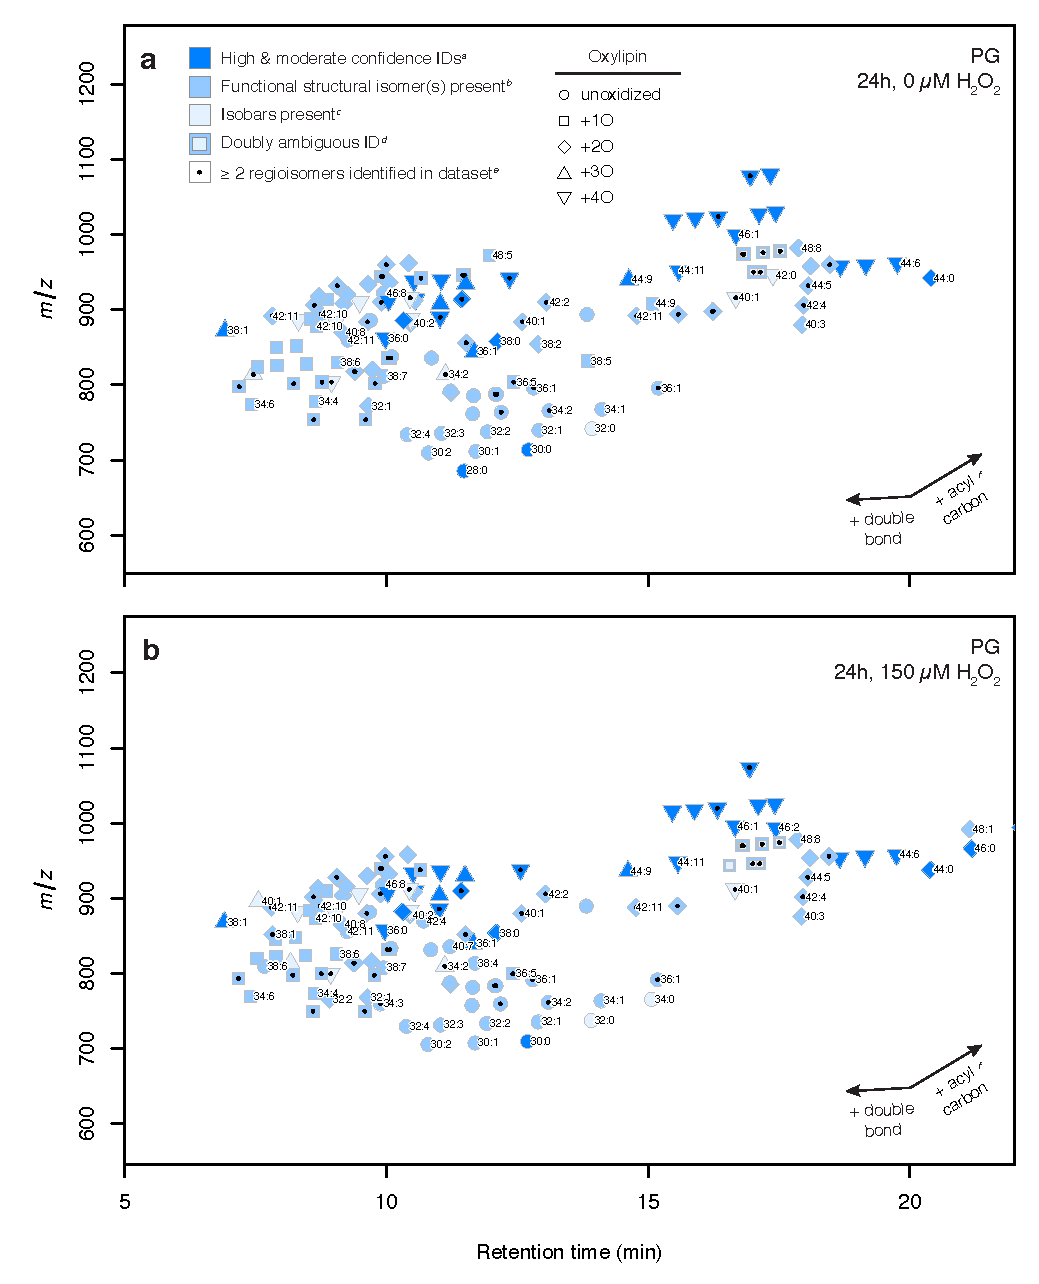
\includegraphics[width=1\textwidth]{Fig_D-8.pdf}
\captionsetup{font={footnotesize}}
\caption[Oxidized and intact species of PG identified in the \emph{P. tricornutum} dataset after 24 hours]{Oxidized and intact species of PG identified in the \emph{P. tricornutum} dataset after 24 hours.}
\label{fig:adn8}
\end{figure}

\clearpage

\begin{figure}[!th]
\centering
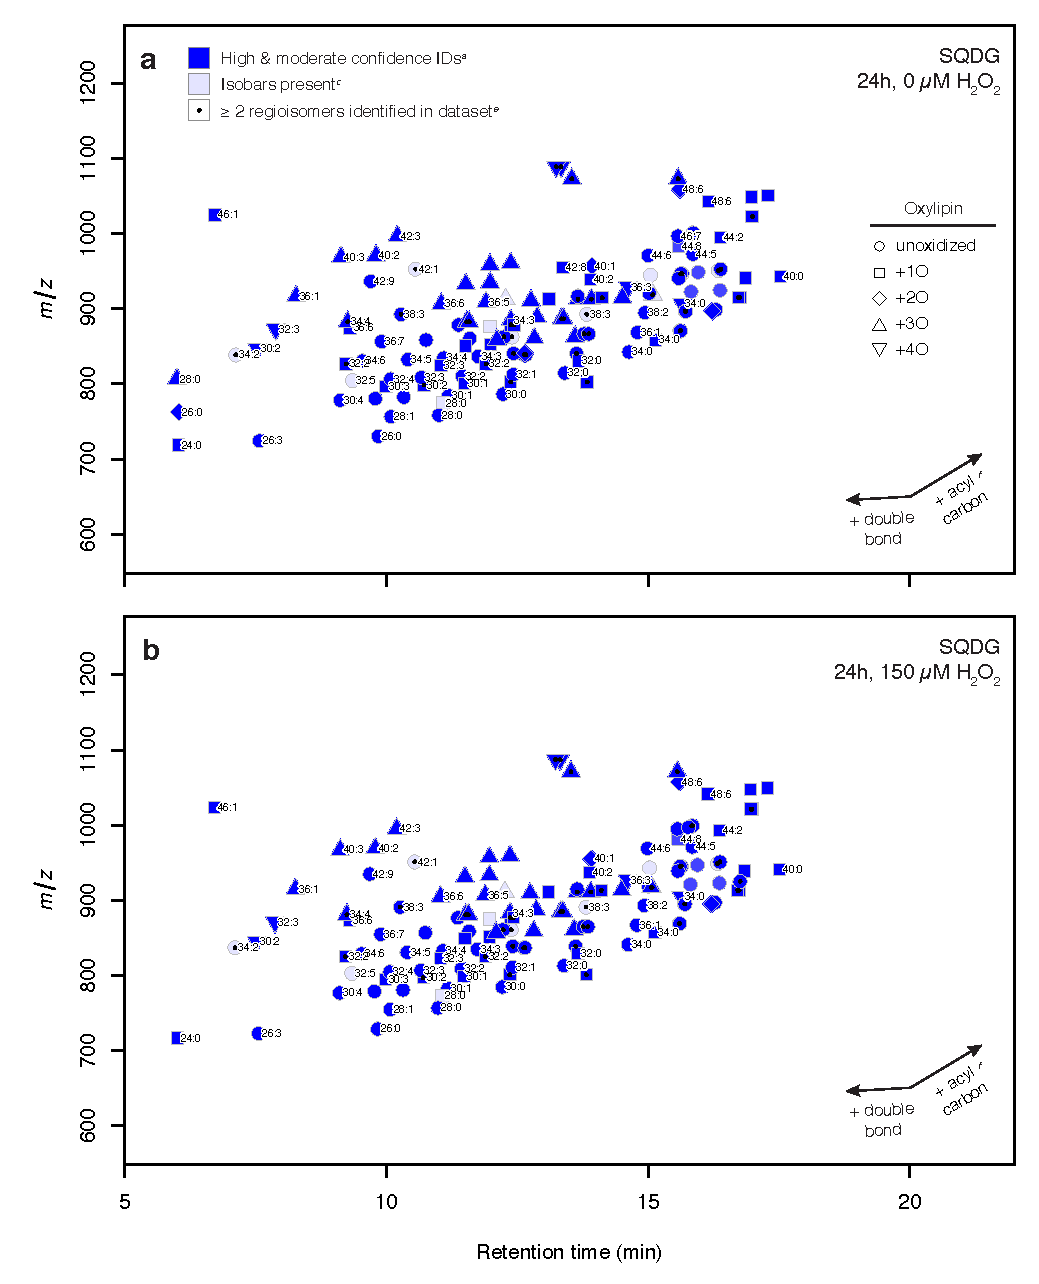
\includegraphics[width=1\textwidth]{Fig_D-9.pdf}
\captionsetup{font={footnotesize}}
\caption[Oxidized and intact species of SQDG identified in the \emph{P. tricornutum} dataset after 24 hours]{Oxidized and intact species of SQDG identified in the \emph{P. tricornutum} dataset after 24 hours.}
\label{fig:adn9}
\end{figure}

\clearpage

\begin{figure}[!th]
\centering
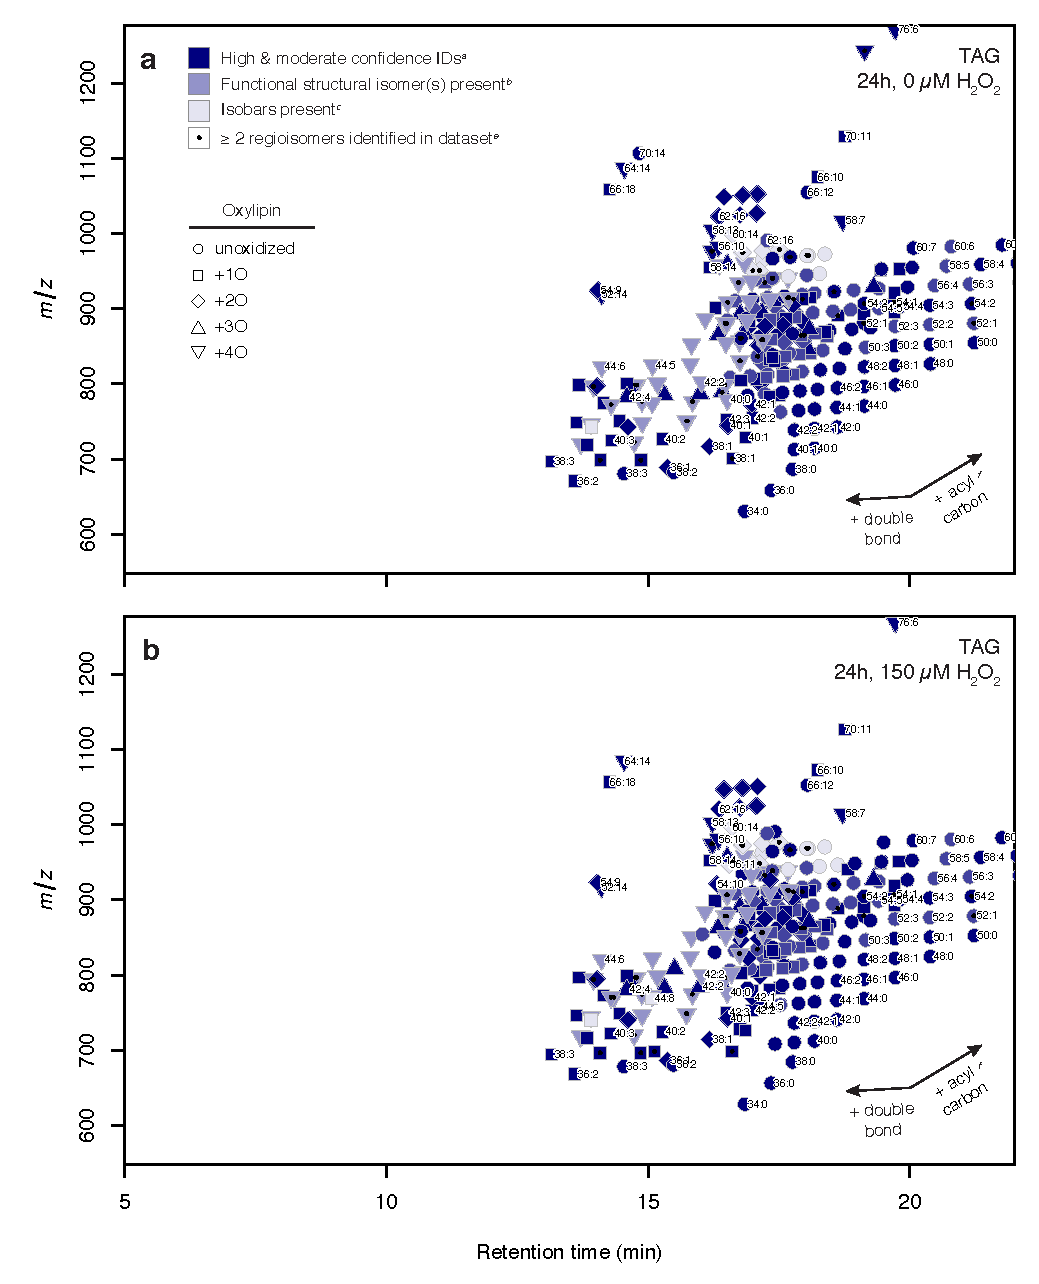
\includegraphics[width=1\textwidth]{Fig_D-10.pdf}
\captionsetup{font={footnotesize}}
\caption[Oxidized and intact species of TAG identified in the \emph{P. tricornutum} dataset after 24 hours]{Oxidized and intact species of TAG identified in the \emph{P. tricornutum} dataset after 24 hours.}
\label{fig:adn10}
\end{figure}

\clearpage

\begin{figure}[!th]
\centering
\includegraphics[width=1\textwidth]{Fig_D-11.pdf}
\end{figure}
\captionsetup{font={footnotesize}}
\captionof{figure}[Expanded version of heatmap in \autoref{fig:c3n3}a]{(preceding page) An expanded version of the heatmap in \autoref{fig:c3n3}a, showing remodeling of the \emph{Phaeodactylum tricornutum} lipidome after 24 h. Heatmap shows relative abundances across two treatments (0 and 150 $\mu$M H\textsubscript{2}O\textsubscript{2}) of all IPL, ox-IPL, and TAG identified by LOBSTAHS with high confidence. Each row (\emph{N} = 896) represents a different compound identified from the database. Heatmap shading shows the relative abundance of each compound as a fold difference of the mean peak area observed in that treatment from the mean peak area of the compound observed across all treatments; grey shading indicates the compound was not observed. Dendrogram clustering and group definitions were determined by similarity profile analysis (Clarke et al., 2008) of lipidome components based on changes in relative peak area across treatments; methodological details are described in the Supporting Information text. To facilitate visualization, each group was randomly assigned a different color; group numbers corresponding to those in \autoref{table:adn8} are also indicated. Solid black lines in the dendrogram indicate branching that was statistically significant (\emph{p} $\leq$ 0.01). \autoref{table:adn8} lists the numbers and identities of the components assigned to each group. Data are presented for a single experiment with two technical replicates.}
\label{fig:adn11}

\clearpage


\section{Supplementary Tables}

\clearpage

\begin{landscape}

\begin{scriptsize}
\begin{singlespace}
\begin{flushleft}
\begin{longtable}{ Lp{.005\linewidth} Lp{.13\linewidth} Lp{.085\linewidth} Lp{.085\linewidth} Lp{.085\linewidth} Lp{.095\linewidth} Lp{.085\linewidth} Lp{.085\linewidth} Lp{.085\linewidth} Lp{.085\linewidth} }
\captionsetup{font={normalsize}}
\caption[Database Dimensions and Ranges of Structural Properties Considered for Each Lipid Class]{Database Dimensions and Ranges of Structural Properties Considered for Each Lipid Class}\\
\label{table:adn1}
\endfirsthead
\endhead
\toprule
\multicolumn{2}{ Lp{.135\linewidth}}{Compound or Compound Class}& \multicolumn{3}{ Lp{.255\linewidth}}{Ranges of Structural Properties Considered in Creation of Database}& No. Unique Compounds & \multicolumn{2}{ Lp{.17\linewidth}}{Number of Adduct Ions\emph{\textsuperscript{a}}}& \multicolumn{2}{ Lp{.17\linewidth}}{Total Database Entries\emph{\textsuperscript{b}}} \\
\cmidrule{3-5}
\cmidrule{7-8}
\cmidrule{9-10}
 &  & Total Acyl Carbon Atoms\emph{\textsuperscript{c}} & Double Bonds\emph{\textsuperscript{c}} & Additional Oxygen Atoms\emph{\textsuperscript{d}} &  & Positive Mode & Negative Mode & Positive Mode & Negative Mode \\
\midrule
\multicolumn{2}{ Lp{.135\linewidth}}{DNP-PE\emph{\textsuperscript{e}}} & --- & --- & --- & 1 & 6 & 5 & 6 & 5 \\
\multicolumn{2}{ Lp{.135\linewidth}}{FFA} & 10-26 & 0-6 & 0-4 & 335 & --- & 1 & 0 & 335 \\
\multicolumn{2}{ Lp{.135\linewidth}}{IP-DAG} &  &  &  &  &  &  &  &  \\
 & DGCC & 20-52 & 0-12 & 0-4 & 1,320 & 5 & 7 & 6,600 & 9,240 \\
 & DGDG & 20-52 & 0-12 & 0-4 & 1,320 & 5 & 7 & 6,600 & 9,240 \\
 & DGTS \& A\emph{\textsuperscript{f}} & 20-52 & 0-12 & 0-4 & 1,320 & 5 & 7 & 6,600 & 9,240 \\
 & MGDG & 20-52 & 0-12 & 0-4 & 1,320 & 5 & 7 & 6,600 & 9,240 \\
 & PC & 20-52 & 0-12 & 0-4 & 1,320 & 5 & 7 & 6,600 & 9,240 \\
 & PE & 20-52 & 0-12 & 0-4 & 1,320 & 5 & 3 & 6,600 & 3,960 \\
 & PG & 20-52 & 0-12 & 0-4 & 1,320 & 6 & 4 & 7,920 & 5,280 \\
 & SQDG & 20-52 & 0-12 & 0-4 & 1,320 & 6 & 3 & 7,920 & 3,960 \\
\multicolumn{2}{ Lp{.135\linewidth}}{Pigments\emph{\textsuperscript{g}}}& --- & --- & --- & 22 & 2 & 6 & 44 & 132 \\
\multicolumn{2}{ Lp{.135\linewidth}}{PUA}& 6-12 & 0-5\emph{\textsuperscript{h}} & 0-4\emph{\textsuperscript{h}} & 155 & 1 & 1 & 155 & 155 \\
\multicolumn{2}{ Lp{.135\linewidth}}{TAG}& 30-78 & 0-18\emph{\textsuperscript{h}} & 0-4 & 2,995 & 7 & --- & 20,965 & 0 \\
\multicolumn{2}{ Lp{.135\linewidth}}{Total}& --- & --- & --- & 14,068 & --- &  & 76,610 & 60,027\\
\bottomrule
\captionsetup{font={footnotesize}}
\caption*{\emph{\textsuperscript{a}} See \autoref{table:adn2}. A blank value indicates the compound or compound class was not typically observed or did not readily form this ion in the given mode.\\
\emph{\textsuperscript{b}} This value reflects all chemically possible combinations of the ranges of properties considered for this compound class.\\
\emph{\textsuperscript{c}} For FFA, IP-DAG, PUA, and TAG.\\
\emph{\textsuperscript{d}} For FFA, IP-DAG, and TAG.\\
\emph{\textsuperscript{e}} Used as internal standard.\\
\emph{\textsuperscript{f}} The betaine lipids DGTS and DGTA are structural isomers; while they can be resolved chromatographically (Popendorf et al., 2013), our current approach requires that they be considered together.\\
\emph{\textsuperscript{g}} The positive mode database contains entries for adduct ions of 22 different common photosynthetic pigments. See \autoref{table:adn3} for definition of abbreviations. The negative mode database includes only chl \emph{a} since pigments are traditionally identified in positive mode (Egeland, 2011).\\
\emph{\textsuperscript{h}} Not all values of these properties were considered for every possible number of total acyl carbon atoms.}
\end{longtable}
\end{flushleft}
\end{singlespace}
\end{scriptsize}

\clearpage

\begin{scriptsize}
\begin{singlespace}
\begin{flushleft}
%\renewcommand*{\arraystretch}{1.3}
\begin{longtable}{ Lp{.01\linewidth} Lp{.1\linewidth} Lp{.005\linewidth} Lp{.045\linewidth} Lp{.045\linewidth} Lp{.045\linewidth} Lp{.045\linewidth} Lp{.045\linewidth} Lp{.045\linewidth} Lp{.045\linewidth} Lp{.045\linewidth} Lp{.045\linewidth} Lp{.045\linewidth} Lp{.045\linewidth} Lp{.045\linewidth} Lp{.045\linewidth}}
\captionsetup{font={normalsize}}
\caption[Relative Abundances for Adduct Ions of Lipid and Oxylipin Species Reported in the Database]{Relative Abundances, by Rank, for Adduct Ions of Lipid and Oxylipin Species Reported in the Database}\\
\label{table:adn2}
\endfirsthead
\endhead
\toprule
 &  &  & Pig-ments\emph{\textsuperscript{a}} & DGCC & DGDG & DGTS \& A\emph{\textsuperscript{b}} & DNP-PE\emph{\textsuperscript{c}} & FFA & MGDG & PC & PE & PG & PUA & SQDG & TAG \\
\midrule
\multicolumn{3}{ Lp{.11\linewidth}}{Positive ion mode} &  &  &  &  &  &  &  &  &  &  &  &  &  \\
 & {[}M+H{]}\textsuperscript{+} &  & 1 & 1 & --- & 1 & 5 & --- & --- & 1 & 1 & 3 & 1 & 4 & --- \\
 & {[}M+K{]}\textsuperscript{+} &  & $\dagger$ & 5 & 3 & 5 & 6 & --- & 4 & 5 & 5 & 6 & --- & 6 & 6 \\
 & {[}M+NH\textsubscript{4}{]}\textsuperscript{+} &  & $\dagger$ & --- & 1 & --- & 1 & --- & 1 & --- & --- & 1 & --- & 1 & 1 \\
 & {[}M+Na{]}\textsuperscript{+} &  & 2 & 2 & 2 & 2 & 2 & --- & 2 & 2 & 2 & 2 & --- & 2 & 2 \\
 & {[}M+2Na-H{]}\textsuperscript{+} &  & $\dagger$ & 4 & 5 & 4 & 3 & --- & 5 & 4 & 3 & 4 & --- & 3 & --- \\
 & {[}M+NH\textsubscript{4}+ACN{]}\textsuperscript{+} &  & $\dagger$ & 3 & 4 & 3 & 4 & --- & 3 & 3 & 4 & 5 & --- & 5 & 4 \\
 & {[}M+2Na+Cl{]}\textsuperscript{+} &  & --- & --- & --- & --- & --- & --- & --- & --- & --- & --- & --- & --- & 5 \\
 & {[}M+C\textsubscript{4}H\textsubscript{10}N\textsubscript{3}{]}\textsuperscript{+} &  & --- & --- & --- & --- & --- & --- & --- & --- & --- & --- & --- & --- & 7 \\
 & {[}M+C\textsubscript{2}H\textsubscript{3}Na\textsubscript{2}O\textsubscript{2}{]}\textsuperscript{+} &  & --- & --- & --- & --- & --- & --- & --- & --- & --- & --- & --- & --- & 3 \\
\multicolumn{3}{ Lp{.11\linewidth}}{Negative ion mode}  &  &  &  &  &  &  &  &  &  &  &  &  &  \\
 & {[}M-H{]}\textsuperscript{-} &  & --- & 7 & 6 & 7 & 1 & 1 & 7 & 7 & 1 & 1 & 1 & 1 & --- \\
 & {[}M+Na-2H{]}\textsuperscript{-} &  & --- & --- & --- & --- & 3 & --- & --- & --- & --- & --- & --- & --- & --- \\
 & {[}M+Cl{]}\textsuperscript{-} &  & 3 & 3 & 2 & 3 & --- & --- & 2 & 3 & --- & --- & $\dagger$ & --- & --- \\
 & {[}M+K-2H{]}\textsuperscript{-} &  & --- & --- & --- & --- & 5 & --- & --- & --- & --- & 4 & --- & --- & --- \\
 & {[}M+HAc-H{]}\textsuperscript{-} &  & 1 & 1 & 1 & 1 & --- & --- & 1 & 1 & --- & --- & $\dagger$ & --- & --- \\
 & {[}M+NaAc-H{]}\textsuperscript{-} &  & --- & --- & --- & --- & 2 & --- & --- & --- & 2 & 2 & --- & 2 & --- \\
 & {[}M+Na+Cl-H{]}\textsuperscript{-} &  & --- & --- & --- & --- & 4 & --- & --- & --- & 3 & 3 & --- & 3 & --- \\
 & {[}M+NaAc+Cl{]}\textsuperscript{-} &  & 5 & 5 & 5 & 5 & --- & --- & 5 & 5 & --- & --- & --- & --- & --- \\
 & {[}M+NaAc+HAc-H{]}\textsuperscript{-} &  & 2 & 2 & 2 & 2 & --- & --- & 3 & 2 & --- & --- & --- & --- & --- \\
 & {[}M+2NaAc+Cl{]}\textsuperscript{-} &  & 6 & 6 & 7 & 6 & --- & --- & 6 & 6 & --- & --- & --- & --- & --- \\
 & {[}M+3Ac+2Na{]}\textsuperscript{-} &  & 4 & 4 & 4 & 4 & --- & --- & 4 & 4 & --- & --- & --- & --- & --- \\
\bottomrule
\captionsetup{font={footnotesize}}
\caption*{Adduct ion abundance rankings were determined empirically using standards under the HPLC-ESI-MS conditions described in the text. To obtain abundance rankings for ox-IPL, we applied the hierarchy observed for the corresponding unoxidized parent IPL. A blank value indicates the compound or compound class was not typically observed or did not readily form this ion in the given mode. A dagger ($\dagger$) indicates that the adduct ion can be observed, but not in a relative abundance that was consistent across samples.\\
\emph{\textsuperscript{a}} The databases contain entries for a range of photosynthetic pigments (see \autoref{table:adn3}).\\
\emph{\textsuperscript{b}} The betaine lipids DGTS and DGTA are structural isomers; while they can be resolved chromatographically (Popendorf et al., 2013), our current approach requires that they be considered together.\\
\emph{\textsuperscript{c}} Used as internal standard.
}
\end{longtable}
\end{flushleft}
\end{singlespace}
\end{scriptsize}
\end{landscape}

\clearpage

\begin{normalsize}
\begin{singlespace}
\begin{flushleft}
%\renewcommand*{\arraystretch}{1.6}x
\begin{longtable}{ Lp{.5\linewidth} Lp{.47\linewidth}}
\captionsetup{font={normalsize}}
\caption[Pigment Abbreviations Used in LOBSTAHS Databases]{Pigment Abbreviations Used in LOBSTAHS Databases}\\
\label{table:adn3}
\endfirsthead
\endhead
\toprule
Pigment & Abbreviation Used in Databases\emph{\textsuperscript{a}} \\
\midrule
$19'$-butanoyloxyfucoxanthin & 19prime\_but\_fuco \\
$19'$-hexanoyloxyfucoxanthin & 19prime\_hex\_fuco \\
Alloxanthin & Allox \\
$\alpha$-carotene & Alpha\_carotene \\
$\beta$-carotenes & Beta\_carotenes \\
Chlorophyll a & Chl\_a \\
Chlorophyll & Chl\_b \\
Chlorophyll c2 & Chl\_c2 \\
Chlorophyll c3 & Chl\_c3 \\
Chlorophyllide a & Chlide\_a \\
Crocoxanthin & Croco \\
Diadinochrome or diadinoxanthin & Dd\_Ddc \\
Diatoxanthin & Dt \\
Echinenone & Echin \\
Fucoxanthin & Fuco \\
Lutein & Lut \\
Neoxanthin or nostoxanthin & Neox\_Nos \\
Peridinin & Peri \\
Pheophytin a & Pheophytin\_a \\
Prasinoxanthin & Pras \\
Violaxanthin & Viol \\
Zeaxanthin & Zeax\\
\bottomrule
\captionsetup{font={footnotesize}}
\caption*{The default LOBSTAHS databases contain entries for adduct ions of 22 different common photosynthetic pigments.\\
\emph{\textsuperscript{a}} If given, this abbreviation is used in the databases in lieu of the full compound name. Abbreviations follow from Egeland (2011). If no abbreviation is given, the full name of the compound is used in the databases. In some cases (e.g., $\alpha$-carotene, $\beta$-carotene, diadinochrome or diadinoxanthin), the database entries for adduct ions of a given pigment will encompass many possible isomers. For each pigment, the databases contain separate entries for the exact masses of multiple adduct ions; in some cases, the relative abundances of these adduct ions are not listed since they were not determined.
}
\end{longtable}
\end{flushleft}
\end{singlespace}
\end{normalsize}

\clearpage

\begin{normalsize}
\begin{singlespace}
\begin{flushleft}
%\renewcommand*{\arraystretch}{1.6}x
\begin{longtable}{ Lp{.45\linewidth} Lp{.25\linewidth} Lp{.25\linewidth}}
\captionsetup{font={normalsize}}
\caption[Retention Time Window Criteria for Various Compounds and Compound Classes]{Retention Time Window Criteria for Various Compounds and Compound Classes}\\
\label{table:adn4}
\endfirsthead
\endhead
\toprule
Lipid Class or Compound\emph{\textsuperscript{a}} & Minimum RT (min.) & Maximum RT (min.) \\
\midrule
DGCC & 7 & 20.4 \\
DGDG & 5 & 19 \\
DGTS \& DGTA & 7 & 20.6 \\
DNP-PE & 14.7 & --- \\
FFA & --- & --- \\
MGDG & 7.1 & 21.1 \\
PC & 6.7 & 20.7 \\
PE & 6.7 & 20.7 \\
PG & 6.7 & 20.7 \\
$19'$-hex-fuco & 10.2 & 10.8 \\
Allox & 10.8 & --- \\
$\beta$-carotenes & 10.8 & --- \\
Chl a & 15.7 & --- \\
Chl b & --- & --- \\
Chl c2 & 5.6 & --- \\
Chlide a & 5.6 & 15.8 \\
Croco & 15.3 & --- \\
Dd or Ddc & 8.5 & --- \\
Dt & --- & --- \\
Echin & 15.3 & --- \\
Fuco & 7.7 & --- \\
Lut & 13.4 & --- \\
Neox or Nos & 8 & --- \\
Peri & --- & --- \\
Pheophytin a & 16.2 & --- \\
Pras & 8 & --- \\
Viol & 8 & --- \\
Zeax & 13.4 & --- \\
SQDG & 6.5 & 18.5 \\
TAG & 15 & 22.7 \\
\bottomrule
\captionsetup{font={footnotesize}}
\caption*{The retention times given in this table are the LOBSTAHS package defaults. RT window data were obtained from authentic standards for representative compounds of each parent lipid class under the chromatographic conditions described in the text. For some compounds or compound classes, minimum or maximum retention times could not be determined. LOBSTAHS users outside of the Van Mooy Lab at WHOI who wish to include screening based on retention time should download a Microsoft Excel spreadsheet included with the package at \url{https://github.com/vanmooylipidomics/LOBSTAHS/} This spreadsheet can be used to generate a table of retention time windows particular to the user's own chromatography; this table can then be imported by specifying a value for rt.windows when calling the function \texttt{doLOBscreen()}.\\
\emph{\textsuperscript{a}} See \autoref{table:adn3} for pigment abbreviations.}
\end{longtable}
\end{flushleft}
\end{singlespace}
\end{normalsize}

\clearpage

\begin{singlespace}
\begin{flushleft}
%\renewcommand*{\arraystretch}{1.6}x
\begin{longtable}{ Lp{.01\linewidth} Lp{.01\linewidth} Lp{.44\linewidth} Lp{.01\linewidth} Lp{.43\linewidth}}
\captionsetup{font={normalsize}}
\caption[xcms, CAMERA, and LOBSTAHS Settings Used in Analysis of the \emph{P. tricornutum} Dataset]{xcms, CAMERA, and LOBSTAHS Settings Used in Analysis of the \emph{P. tricornutum} Dataset}\\
\label{table:adn5}
\endfirsthead
\endhead
\toprule
\multicolumn{3}{ l }{Parameter}  &  & Value \\
\midrule
\multicolumn{3}{ l }{xcms}&  &  \\
 & \multicolumn{2}{ l }{\texttt{xcmsSet()}} &  &  \\
 &  & method &  & centWave \\
 &  & profparam\emph{\textsuperscript{a}} &  & list(step=0.001) \\
 &  & ppm &  & 2.5 \\
 &  & min./max. peakwidth\emph{\textsuperscript{b}} &  & 35, 88 \\
 &  & fitgauss &  & TRUE \\
 &  & noise &  & 500 \\
 &  & mzdiff\emph{\textsuperscript{b}} &  & 0.002432 \\
 &  & verbose.columns &  & TRUE \\
 &  & snthresh &  & 10 \\
 &  & integrate &  & 1 \\
 &  & prefilter\emph{\textsuperscript{b}} &  & 3, 19000 \\
 &  & mzCenterFun &  & wMean \\
 & \multicolumn{2}{ l }{\texttt{group()}\emph{\textsuperscript{c}}}&  &  \\
 &  & method &  & density \\
 &  & bw\emph{\textsuperscript{b}} &  & 15 \\
 &  & minfrac\emph{\textsuperscript{b}} &  & 0.38 \\
 &  & minsamp &  & 2 \\
 &  & mzwid\emph{\textsuperscript{b}} &  & 0.001 \\
 &  & max &  & 50 \\
 & \multicolumn{2}{ l }{\texttt{retcor()}} &  &  \\
 &  & method &  & loess \\
 &  & missing\emph{\textsuperscript{b}} &  & 3 \\
 &  & extra\emph{\textsuperscript{b}} &  & 1 \\
 &  & smooth &  & loess \\
 &  & span\emph{\textsuperscript{b}} &  & 0.3 \\
 &  & family &  & gaussian \\
 & \multicolumn{2}{ l }{\texttt{fillPeaks()}} &  &  \\
 &  & method &  & chrom \\
\multicolumn{3}{ l }{CAMERA}  &  &  \\
 & \multicolumn{2}{ l }{\texttt{annotate()}} &  &  \\
 &  & quick &  & FALSE \\
 &  & sample &  & NA \\
 &  & sigma &  & 6 \\
 &  & perfwhm &  & 0.6 \\
 &  & cor\_eic\_th &  & 0.75 \\
 &  & graphMethod &  & hcs \\
 &  & pval &  & 0.05 \\
 &  & calcCiS &  & TRUE \\
 &  & calcIso &  & TRUE \\
 &  & calcCaS &  & FALSE \\
 &  & maxcharge &  & 4 \\
 &  & maxiso &  & 0.5 \\
 &  & minfrac &  & 0.5 \\
 &  & psg\_list &  & NULL \\
 &  & rules &  & NULL \\
 &  & polarity &  & positive \\
 &  & multiplier &  & 3 \\
 &  & max\_peaks &  & 100 \\
 &  & intval &  & into \\
 &  & ppm &  & 2.5 \\
 &  & mzabs &  & 0.0015 \\
\multicolumn{3}{ l }{LOBSTAHS} &  &  \\
 & \multicolumn{2}{ l }{\texttt{doLOBscreen()}} &  &  \\
 &  & polarity &  & positive \\
 &  & database &  & NULL\emph{\textsuperscript{d}} \\
 &  & remove.iso &  & TRUE \\
 &  & rt.restrict &  & TRUE \\
 &  & rt.windows &  & NULL\emph{\textsuperscript{d}} \\
 &  & exclude.oddFA &  & TRUE \\
 &  & match.ppm &  & 2.5\\
\bottomrule
\captionsetup{font={footnotesize}}
\caption*{The R script \href{https://github.com/vanmooylipidomics/LipidomicsToolbox/blob/master/prepOrbidata.R}{prepOrbidata.R} can be used to apply the xcms and CAMERA settings presented here in a single sequence. The is not part of the LOBSTAHS R package, but can be downloaded as part of the Van Mooy Lab Lipidomics Toolbox from \url{https://github.com/vanmooylipidomics/LipidomicsToolbox/}\\
\emph{\textsuperscript{a}} Because the mass accuracy of the Orbitrap can surpass the width of the \emph{m/z} windows used to define each peak, a very small value should be used for profparam.\\
\emph{\textsuperscript{b}} Values for these parameters were optimized using the IPO package (Libiseller et al., 2015). Where applicable, we used the values in Table 1 of Patti et al. (2012) as initial values for IPO optimization.\\
\emph{\textsuperscript{c}} The \texttt{group()} function was applied to the data twice: Once after \texttt{xcmsSet()} and then again after \texttt{retcor()}. The parameter values given here were used in both instances.\\
\emph{\textsuperscript{d}} \texttt{doLOBscreen()} applies the LOBSTAHS package defaults when NULL (or no value) is specified for these parameters. The default database is described in \autoref{table:adn1} and \autoref{table:adn2}, while the default retention time windows are described in \autoref{table:adn4}.}
\end{longtable}
\end{flushleft}
\end{singlespace}

\clearpage

\begin{landscape}

\begin{footnotesize}
\begin{singlespace}
%\renewcommand*{\arraystretch}{1.6}
\begin{longtable}{ Lp{.08\linewidth} Lp{.07\linewidth} Lp{.07\linewidth} Lp{.08\linewidth} Lp{.08\linewidth} Lp{.08\linewidth} Lp{.08\linewidth} Lp{.08\linewidth} Lp{.11\linewidth} Lp{.1\linewidth} }
\captionsetup{font={normalsize}}
\caption[Evaluation of Method Performance using Alternative Software]{Evaluation of Method Performance using IPL standards and Alternative Software for Feature Detection and Chromatographic Alignment}\\
\label{table:adn6}
\endfirsthead
\endhead
\toprule
Lipid Class & Origin of Standard & Moieties Present in Standard\emph{\textsuperscript{a}} & Dominant Positive Mode Adduct Ion & Ion Exact \emph{m/z} & Observed \emph{m/z}\emph{\textsuperscript{b}} & Rel. Mass Uncertainty (ppm)\emph{\textsuperscript{c}} & Correct LOBSTAHS ID? & Confidence in Assignment After Adduct Hierarchy Screening\emph{\textsuperscript{d}} & Structural Isomers or Isobars Present After Screening? \\
\midrule
MGDG & Natural & 34:0 & {[}M+NH\textsubscript{4}{]}\textsuperscript{+} & 776.6246 & 776.6248 & 0.2 & Yes & High confidence & No \\
 &  & 36:0 & {[}M+NH\textsubscript{4}{]}\textsuperscript{+} & 804.6559 & 804.6559 & 0.02 & Yes & High confidence & No \\
DNP-PE & Synthetic & 32:0 & {[}M+NH\textsubscript{4}{]}\textsuperscript{+} & 875.5505 & 875.5507 & 0.2 & Yes & High confidence & No \\
SQDG & Natural & 34:3 & {[}M+NH\textsubscript{4}{]}\textsuperscript{+} & 834.5396 & 834.5397 & 0.2 & Yes & High confidence & No \\
 &  & 34:2 & {[}M+NH\textsubscript{4}{]}\textsuperscript{+} & 836.5552 & 836.5554 & 0.2 & Yes & High confidence & No \\
PG & Synthetic & 32:0 & {[}M+NH\textsubscript{4}{]}\textsuperscript{+} & 740.5436 & 740.5438 & 0.3 & Yes & High confidence & No \\
PE & Synthetic & 32:0 & {[}M+H{]}\textsuperscript{+} & 692.5225 & 692.5227 & 0.3 & Yes & High confidence & No \\
PC & Synthetic & 32:0 & {[}M+H{]}\textsuperscript{+} & 734.5694 & 734.5695 & 0.1 & Yes & High confidence & No \\
DGDG & Natural & 34:2 & {[}M+NH\textsubscript{4}{]}\textsuperscript{+} & 934.6461 & 934.6463 & 0.1 & Yes & High confidence & No \\
 &  & 36:4 & {[}M+NH\textsubscript{4}{]}\textsuperscript{+} & 958.6461 & 958.6463 & 0.1 & Yes & High confidence & No \\
Mean &  &  &  &  &  & 0.2 &  &  & \\
\bottomrule
\captionsetup{font={footnotesize}}
\caption*{The results in this table were obtained as in \autoref{table:c3n1} in the text, except that MAVEN (Clasquin et al., 2012; Melamud et al., 2010) was used instead of xcms for initial peak picking (feature detection) and chromatographic alignment.\\
\emph{\textsuperscript{a}} Multiple moieties were present in glycolipid standards purified from natural samples; in these cases, only predominant moieties are shown\\
\emph{\textsuperscript{b}} Mean observed \emph{m/z} ratio in 5 independent samples\\
\emph{\textsuperscript{c}} $\left| {\frac{{{\text{Observed exact mass}} - {\text{Database exact mass}}}}{{{\text{Database exact mass}}}}} \right| \times {10^6}$\\	
\emph{\textsuperscript{d}} ``High confidence'' indicates the assignment fully satisfied all adduct hierarchy rules and other screening criteria applied as described in the text.
}
\end{longtable}
\end{singlespace}
\end{footnotesize}

\clearpage

\begin{footnotesize}
\begin{singlespace}
\begin{flushleft}
%\renewcommand*{\arraystretch}{1.6}x
\begin{longtable}{ Lp{.12\linewidth} Lp{.09\linewidth} Lp{.09\linewidth} Lp{.09\linewidth} Lp{.09\linewidth} Lp{.09\linewidth} Lp{.09\linewidth} Lp{.09\linewidth} Lp{.09\linewidth} }
\captionsetup{font={normalsize}}
\caption[Annotation of Isomers and Isobars in Screened \emph{P. tricornutum} Dataset]{Annotation of Isomers and Isobars in Screened \emph{P. tricornutum} Dataset}\\
\label{table:adn7}
\endfirsthead
\endhead
\toprule
 & \multicolumn{2}{ Lp{.18\linewidth} }{Peaks (Features) for which Isomer/Isobar Type was Identified} & \multicolumn{2}{ Lp{.18\linewidth} }{Peak Groups in which Isomer/Isobar Type was Identified} & \multicolumn{2}{ Lp{.18\linewidth} }{Assignments for which Isomer/Isobar Type was Identified} & \multicolumn{2}{ Lp{.18\linewidth} }{Parent Compounds for which Isomer/Isobar Type Was Identified}  \\
\cmidrule{2-9}
Type of Feature & No. & \% Total Peaks & No. & \% Total Peak Groups & No. & \% Total Assignments & No. & \% Total Parent Compounds \\
\midrule
Functional structural isomer & 5,057 & 23 & 375 & 24 & 752 & 37 & 577 & 29 \\
Isobar & 1,137 & 5 & 84 & 5 & 195 & 9 & 162 & 8 \\
Any ambiguity\emph{\textsuperscript{a}} & 5,401 & 25 & 432 & 27 & 893 & 43 & 699 & 36 \\
Regioisomer & 7,591 & 35 & 556 & 35 & 750 & 36 & 352 & 18\\
\bottomrule
\captionsetup{font={footnotesize}}
\caption*{\emph{\textsuperscript{a}} Elements having either a functional structural isomer, isobar, or both.}
\end{longtable}
\end{flushleft}
\end{singlespace}
\end{footnotesize}

\clearpage

\begin{footnotesize}
\begin{singlespace}
\begin{flushleft}
%\renewcommand*{\arraystretch}{1.6}x
\begin{longtable}{ Lp{.03\linewidth} Lp{.12\linewidth} Lp{.03\linewidth} Lp{.24\linewidth} Lp{.24\linewidth} Lp{.24\linewidth} }
\captionsetup{font={normalsize}}
\caption[List of Groups of \emph{P. Tricornutum} Lipidome Components Determined by Similarity Profile Analysis]{List of Groups of \emph{P. Tricornutum} Lipidome Components Determined by Similarity Profile Analysis in 0 $\mu$m and 150 $\mu$m H\textsubscript{2}O\textsubscript{2} Treatments at 24 h}\\
\label{table:adn8}
\endfirsthead
\endhead
\toprule
Group No. & Abundance of Group Components in 150 $\mu$M H\textsubscript{2}O\textsubscript{2} Treatment Relative to 0 $\mu$M Control\emph{\textsuperscript{a}} & No. Components & \multicolumn{3}{ l }{Component Molecules Assigned by Similarity Profile Analysis}  \\
\midrule
1 & \multirow{2}{2.7cm}[0em]{Less abundant (downregulated)} & 30 & MGDG 42:4 +1O, RT 11.33 min & TAG 70:14, RT 14.83 min & PG 42:11 +3O, RT 11.01 min \\
 &  &  & DGDG 40:1 +1O, RT 17.75 min & DGDG 36:8 +1O, RT 14.1 min & PE 32:5 +1O, RT 6.36 min \\
 &  &  & DGDG 36:1 +1O, RT 16.84 min & DGDG 36:8 +1O, RT 11.64 min & DGDG 36:9, RT 14.05 min \\
 &  &  & PE 44:5, RT 12.09 min & TAG 70:11 +1O, RT 18.76 min & SQDG 30:2 +4O, RT 7.52 min \\
 &  &  & SQDG 36:1 +3O, RT 8.26 min & MGDG 46:5 +1O, RT 17.17 min & PE 42:4, RT 11.6 min \\
 &  &  & PE 40:7 +4O, RT 8.65 min & SQDG 32:3 +2O, RT 12.63 min & PE 40:2, RT 12.82 min \\
 &  &  & PE 42:9 +1O, RT 9.22 min & MGDG 38:0 +2O, RT 18.04 min & MGDG 38:6, RT 10.51 min \\
 &  &  & PE 38:7 +1O, RT 8.5 min & TAG 66:10 +1O, RT 18.23 min & MGDG 48:8 +1O, RT 16.46 min \\
 &  &  & PE 36:5 +1O, RT 8.82 min & TAG 58:7 +4O, RT 18.71 min & DGCC 40:0 +4O, RT 16.36 min \\
 &  &  & MGDG 30:6, RT 9.59 min & DGDG 44:8 +1O, RT 16.22 min & PE 40:9 +1O, RT 8.26 min \\
2 & \multirow{2}{2.7cm}[0em]{More abundant (upregulated)} & 105 & TAG 52:13 +1O, RT 14.54 min & MGDG 40:6 +2O, RT 15.65 min & PE 40:1 +1O, RT 17.28 min \\
 &  &  & TAG 56:3 +2O, RT 18.82 min & TAG 44:4 +3O, RT 15.51 min & PE 52:3 +4O, RT 17.3 min \\
 &  &  & MGDG 42:7 +1O, RT 16.89 min & PE 34:1, RT 15.6 min & TAG 56:7 +4O, RT 17.23 min \\
 &  &  & MGDG 40:3 +2O, RT 16.9 min & DGDG 36:5 +2O, RT 10.55 min & PE 48:8 +1O, RT 8.37 min \\
 &  &  & MGDG 34:2 +1O, RT 16.89 min & TAG 56:15, RT 16.23 min & TAG 48:11, RT 15.7 min \\
 &  &  & MGDG 36:6 +1O, RT 6.53 min & TAG 52:10 +1O, RT 16.18 min & DGDG 48:8, RT 7.36 min \\
 &  &  & TAG 56:13 +1O, RT 15.93 min & TAG 50:8 +2O, RT 16.18 min & PE 42:4 +2O, RT 7.43 min \\
 &  &  & TAG 52:10 +2O, RT 15.88 min & TAG 50:9 +1O, RT 16.18 min & MGDG 44:6 +3O, RT 16.6 min \\
 &  &  & MGDG 38:4 +2O, RT 15.9 min & TAG 50:11, RT 16.27 min & MGDG 36:1 +2O, RT 16.74 min \\
 &  &  & TAG 50:12, RT 15.87 min & TAG 48:10, RT 16.13 min & MGDG 34:0 +2O, RT 16.69 min \\
 &  &  & DGDG 42:1 +2O, RT 9.59 min & MGDG 48:7 +3O, RT 15.22 min & SQDG 42:0, RT 16.66 min \\
 &  &  & DGDG 38:9 +2O, RT 8.68 min & MGDG 40:7 +2O, RT 15.17 min & PE 46:1 +4O, RT 16.66 min \\
 &  &  & DGDG 36:9 +2O, RT 7.95 min & TAG 38:1 +1O, RT 15.12 min & PG 42:0 +2O, RT 16.66 min \\
 &  &  & PC 48:8 +2O, RT 8.97 min & TAG 48:12, RT 15.14 min & MGDG 38:5 +1O, RT 16.66 min \\
 &  &  & PG 44:1 +4O, RT 8.97 min & TAG 50:7 +2O, RT 16.51 min & TAG 52:14, RT 15.41 min \\
 &  &  & DGDG 36:1, RT 8.48 min & MGDG 34:3 +1O, RT 16.52 min & MGDG 40:4 +1O, RT 11.91 min \\
 &  &  & DGDG 32:3 +1O, RT 9.64 min & MGDG 40:5 +2O, RT 15.96 min & MGDG 42:7 +3O, RT 17.09 min \\
 &  &  & MGDG 32:6 +1O, RT 8.37 min & MGDG 46:5 +1O, RT 16.02 min & PE 44:4 +1O, RT 17.14 min \\
 &  &  & MGDG 24:3 +1O, RT 9.53 min & TAG 46:9, RT 16.09 min & PE 42:3 +1O, RT 17.09 min \\
 &  &  & MGDG 48:6 +3O, RT 15.73 min & TAG 48:7 +2O, RT 16 min & TAG 54:9 +1O, RT 17.09 min \\
 &  &  & MGDG 42:3 +1O, RT 15.74 min & TAG 64:17, RT 17.38 min & TAG 42:4, RT 17.13 min \\
 &  &  & TAG 52:11 +1O, RT 15.77 min & PE 48:2 +4O, RT 16.8 min & TAG 42:4, RT 17.09 min \\
 &  &  & TAG 50:9 +2O, RT 15.79 min & PC 44:9 +4O, RT 16.8 min & PE 48:2 +1O, RT 17.84 min \\
 &  &  & MGDG 36:6 +1O, RT 15.7 min & MGDG 44:9 +3O, RT 16.78 min & PE 46:0 +1O, RT 18.02 min \\
 &  &  & DGDG 36:5 +1O, RT 13.18 min & PG 42:2 +4O, RT 16.8 min & PG 46:2 +4O, RT 17.44 min \\
 &  &  & PC 32:3 +1O, RT 9.85 min & MGDG 42:4 +3O, RT 16.81 min & PE 44:1 +2O, RT 20.39 min \\
 &  &  & MGDG 42:8 +2O, RT 15.31 min & MGDG 36:0 +3O, RT 16.77 min & TAG 64:16, RT 17.53 min \\
 &  &  & TAG 36:1 +1O, RT 13.83 min & TAG 44:6, RT 16.77 min & MGDG 44:4 +1O, RT 15.86 min \\
 &  &  & MGDG 36:9 +4O, RT 7.02 min & TAG 56:11 +1O, RT 16.95 min & SQDG 30:2 +1O, RT 8.39 min \\
 &  &  & DGDG 46:7 +4O, RT 14.66 min & MGDG 40:6 +3O, RT 16.95 min & MGDG 38:4 +3O, RT 15.76 min \\
 &  &  & MGDG 36:8 +1O, RT 11.35 min & MGDG 38:1 +3O, RT 16.94 min & MGDG 32:2 +2O, RT 10.36 min \\
 &  &  & DGDG 36:7 +1O, RT 11.19 min & PE 44:2 +1O, RT 16.99 min & MGDG 40:7 +1O, RT 16.47 min \\
 &  &  & MGDG 24:3, RT 11.78 min & DGDG 44:2 +1O, RT 17.32 min & PE 40:2 +1O, RT 16.95 min \\
 &  &  & MGDG 40:4 +3O, RT 16.39 min & PE 50:1 +4O, RT 17.37 min & SQDG 38:4 +4O, RT 17.47 min \\
 &  &  & TAG 44:7, RT 16.43 min & PE 44:1 +1O, RT 17.35 min & TAG 52:11 +2O, RT 15.3 min \\
3 & More abundant & 11 & TAG 54:12, RT 16.87 min & TAG 54:8 +1O, RT 17.43 min & TAG 56:13, RT 16.99 min \\
 &  &  & SQDG 40:1 +2O, RT 13.91 min & TAG 52:10, RT 17.14 min & TAG 52:8 +1O, RT 16.94 min \\
 &  &  & DGDG 32:2 +2O, RT 9.65 min & TAG 52:5 +2O, RT 17.76 min & SQDG 36:6 +1O, RT 9.29 min \\
 &  &  & TAG 46:7, RT 16.9 min & TAG 52:11, RT 16.78 min &  \\
4 & More abundant & 8 & TAG 42:2 +3O, RT 15.99 min & TAG 50:6 +2O, RT 16.91 min & TAG 50:5 +2O, RT 17.23 min \\
 &  &  & SQDG 32:2 +1O, RT 9.22 min & TAG 58:13, RT 17.38 min & MGDG 42:1 +1O, RT 13.98 min \\
 &  &  & PE 46:1 +1O, RT 17.75 min & MGDG 36:0 +2O, RT 16.94 min &  \\
5 & More abundant & 9 & TAG 60:14, RT 17.37 min & TAG 42:4 +3O, RT 14.59 min & SQDG 40:2 +1O, RT 13.88 min \\
 &  &  & MGDG 40:5 +1O, RT 17.12 min & TAG 54:11, RT 17.2 min & PE 46:3 +1O, RT 17.83 min \\
 &  &  & PG 38:1 +3O, RT 6.9 min & TAG 52:9, RT 17.47 min & MGDG 46:8 +1O, RT 17.35 min \\
6 & More abundant & 4 & TAG 48:4 +1O, RT 17.38 min & TAG 50:1, RT 20.39 min & TAG 52:4, RT 19.25 min \\
 &  &  & TAG 46:4, RT 17.9 min &  &  \\
7 & More abundant & 4 & SQDG 40:7 +3O, RT 12.36 min & TAG 52:5, RT 18.89 min & MGDG 46:7 +1O, RT 17.68 min \\
 &  &  & MGDG 32:5 +2O, RT 8.73 min &  &  \\
8 & More abundant & 5 & TAG 50:0, RT 21.23 min & TAG 44:3, RT 17.87 min & PC 40:1, RT 14.58 min \\
 &  &  & DGTS\_DGTA 40:1, RT 18.08 min & PC 36:2, RT 15.71 min &  \\
9 & More abundant & 5 & MGDG 44:1 +1O, RT 19.46 min & PG 44:0 +2O, RT 20.39 min & PE 42:10, RT 12.6 min \\
 &  &  & TAG 44:6 +1O, RT 14.15 min & TAG 54:2, RT 19.13 min &  \\
10 & More abundant & 6 & TAG 44:0, RT 19.13 min & DGDG 32:5, RT 10.56 min & TAG 56:8, RT 18.55 min \\
 &  &  & PE 40:2 +2O, RT 14.36 min & MGDG 36:9 +2O, RT 8.43 min & TAG 42:1, RT 18.18 min \\
11 & More abundant & 9 & TAG 44:2 +1O, RT 17.32 min & PE 38:1 +2O, RT 14.24 min & PC 44:4, RT 17.65 min \\
 &  &  & TAG 52:6 +1O, RT 17.63 min & PC 46:8 +4O, RT 17.57 min & PE 42:5 +2O, RT 12.74 min \\
 &  &  & TAG 52:8, RT 17.75 min & DGDG 48:4 +1O, RT 17.42 min & TAG 48:5 +1O, RT 17.33 min \\
12 & More abundant & 7 & MGDG 44:4 +1O, RT 18.18 min & TAG 52:1, RT 19.12 min & MGDG 42:4 +1O, RT 17.81 min \\
 &  &  & PE 40:4 +2O, RT 12.34 min & MGDG 36:9 +1O, RT 8.8 min & TAG 54:3 +1O, RT 19.71 min \\
 &  &  & DGDG 32:5, RT 10.46 min &  &  \\
13 & More abundant & 6 & PC 44:4, RT 17.76 min & SQDG 34:4 +3O, RT 9.25 min & TAG 42:3 +3O, RT 15.31 min \\
 &  &  & TAG 56:11, RT 17.6 min & DGTS\_DGTA 38:7, RT 14.32 min & TAG 42:1 +3O, RT 16.41 min \\
14 & More abundant & 3 & TAG 48:6, RT 17.6 min & PC 48:8 +1O, RT 8.07 min & TAG 58:1, RT 24.67 min \\
15 & More abundant & 9 & TAG 46:4 +1O, RT 17.07 min & MGDG 42:3 +4O, RT 15.13 min & DGDG 36:7 +2O, RT 8.8 min \\
 &  &  & DGTS\_DGTA 30:0, RT 14.5 min & PC 34:0, RT 16.42 min & TAG 54:1, RT 19.69 min \\
 &  &  & MGDG 44:6 +3O, RT 17.76 min & PC 32:0, RT 15.4 min & TAG 42:2, RT 17.79 min \\
16 & More abundant & 8 & PC 38:5, RT 15.73 min & TAG 46:0, RT 19.72 min & TAG 60:13, RT 17.71 min \\
 &  &  & TAG 46:5, RT 17.56 min & PC 34:0, RT 16.45 min & MGDG 38:9 +2O, RT 9.26 min \\
 &  &  & DGTS\_DGTA 44:12, RT 6.67 min & TAG 48:6 +1O, RT 17.41 min &  \\
17 & More abundant & 7 & PC 42:11 +1O, RT 9.84 min & TAG 54:7 +1O, RT 17.95 min & TAG 48:4 +2O, RT 17.11 min \\
 &  &  & TAG 50:8, RT 17.38 min & TAG 60:5, RT 21.76 min & TAG 46:5 +1O, RT 16.77 min \\
 &  &  & PC 32:2 +1O, RT 10.74 min &  &  \\
18 & More abundant & 10 & PC 36:9 +1O, RT 8.09 min & TAG 50:2 +2O, RT 17.95 min & TAG 50:4 +2O, RT 17.57 min \\
 &  &  & TAG 44:1 +2O, RT 17.14 min & TAG 42:5 +1O, RT 13.64 min & TAG 48:0, RT 20.39 min \\
 &  &  & DGDG 48:3 +1O, RT 17.79 min & MGDG 36:7 +2O, RT 9.62 min & DGTS\_DGTA 42:2, RT 17.94 min \\
 &  &  & PE 42:1 +1O, RT 17.69 min &  &  \\
19 & Less abundant & 13 & PC 34:7 +1O, RT 7.95 min & PG 36:0 +4O, RT 9.97 min & DGDG 44:11, RT 13.57 min \\
 &  &  & PC 36:8 +1O, RT 8.2 min & MGDG 34:7, RT 8.16 min & PE 38:3 +1O, RT 11.65 min \\
 &  &  & PE 30:1 +1O, RT 9.79 min & MGDG 40:10, RT 12.13 min & PE 42:7 +4O, RT 9.52 min \\
 &  &  & PE 42:0 +4O, RT 9.99 min & MGDG 44:10 +2O, RT 8.22 min & PE 36:6 +1O, RT 8.05 min \\
 &  &  & PC 34:6 +1O, RT 8.5 min &  &  \\
20 & More abundant & 3 & DGTS\_DGTA 50:3, RT 19.7 min & DGDG 34:5, RT 11.83 min & DGTS\_DGTA 42:0, RT 18.89 min \\
21 & More abundant & 5 & PC 40:1, RT 18.01 min & SQDG 32:0 +1O, RT 13.66 min & DGDG 40:1, RT 17.42 min \\
 &  &  & PE 48:3 +4O, RT 11.01 min & MGDG 36:8 +2O, RT 9.01 min &  \\
22 & More abundant & 3 & PG 38:0 +2O, RT 12.11 min & TAG 58:2, RT 23.2 min & PC 44:5, RT 13.37 min \\
23 & More abundant & 3 & MGDG 34:5, RT 8.22 min & DGTS\_DGTA 40:7, RT 14.31 min & DGTS\_DGTA 42:4, RT 17.22 min \\
24 & More abundant & 2 & TAG 54:2, RT 21.18 min & TAG 54:2, RT 21.18 min & TAG 54:2, RT 21.18 min \\
 &  &  & TAG 54:2, RT 21.18 min & TAG 54:4, RT 19.81 min &  \\
25 & More abundant & 4 & PC 36:1, RT 16.47 min & DGTS\_DGTA 36:1, RT 16.82 min & DGTS\_DGTA 44:5, RT 17.43 min \\
 &  &  & MGDG 26:1 +4O, RT 16.47 min &  &  \\
26 & More abundant & 4 & SQDG 34:2 +3O, RT 13.33 min & DGTS\_DGTA 42:7, RT 15.37 min & SQDG 34:2 +3O, RT 13.37 min \\
 &  &  & MGDG 42:7 +1O, RT 10.45 min &  &  \\
27 & More abundant & 1 & SQDG 46:1 +1O, RT 6.71 min & SQDG 46:1 +1O, RT 6.71 min & SQDG 46:1 +1O, RT 6.71 min \\
 &  &  & SQDG 46:1 +1O, RT 6.71 min &  &  \\
28 & More abundant & 5 & PE 40:8, RT 13.23 min & TAG 56:2, RT 22.1 min & PE 34:0 +2O, RT 12.51 min \\
 &  &  & PC 42:3, RT 14.33 min & PE 38:3 +4O, RT 12.51 min &  \\
29 & More abundant & 3 & PC 30:4, RT 10.52 min & DGTS\_DGTA 40:2, RT 17.42 min & DGDG 34:5, RT 11.81 min \\
30 & More abundant & 6 & DGTS\_DGTA 38:3, RT 16.08 min & TAG 46:7 +1O, RT 14.6 min & PC 38:6, RT 13.67 min \\
 &  &  & MGDG 36:8 +1O, RT 9.04 min & PC 42:10, RT 12.38 min & PC 40:7, RT 13.75 min \\
31 & NS\emph{\textsuperscript{b}} & 2 & PC 32:6, RT 9.89 min & PC 32:6, RT 9.89 min & PC 32:6, RT 9.89 min \\
 &  &  & PC 32:6, RT 9.89 min & TAG 38:2 +1O, RT 14.09 min &  \\
32 & More abundant & 5 & TAG 74:6 +4O, RT 19.13 min & SQDG 36:4 +1O, RT 12.42 min & PC 38:7, RT 13.91 min \\
 &  &  & PC 36:7 +1O, RT 8.92 min & TAG 38:2, RT 15.49 min &  \\
33 & More abundant & 2 & PC 36:4, RT 13.96 min & PC 36:4, RT 13.96 min & PC 36:4, RT 13.96 min \\
 &  &  & PC 36:4, RT 13.96 min & PC 40:5, RT 15.71 min &  \\
34 & More abundant & 4 & DGDG 32:4, RT 11.28 min & TAG 40:3 +1O, RT 14.3 min & SQDG 36:4 +1O, RT 12.37 min \\
 &  &  & PC 38:3, RT 15.9 min &  &  \\
35 & More abundant & 1 & TAG 50:4 +3O, RT 17.18 min & TAG 50:4 +3O, RT 17.18 min & TAG 50:4 +3O, RT 17.18 min \\
 &  &  & TAG 50:4 +3O, RT 17.18 min &  &  \\
36 & More abundant & 4 & PE 38:4, RT 13.23 min & TAG 58:3, RT 22.05 min & DGTS\_DGTA 44:1, RT 18.94 min \\
 &  &  & DGDG 34:1, RT 15.27 min &  &  \\
37 & More abundant & 3 & DGTS\_DGTA 34:3, RT 14.02 min & DGDG 40:10, RT 11.38 min & SQDG 36:3 +3O, RT 13.9 min \\
38 & More abundant & 6 & TAG 40:2 +2O, RT 14.62 min & MGDG 36:10, RT 10.66 min & PC 36:9, RT 10 min \\
 &  &  & DGDG 34:4, RT 12.74 min & DGTS\_DGTA 34:6, RT 12.94 min & DGTS\_DGTA 40:5, RT 16 min \\
39 & More abundant & 4 & DGDG 34:6, RT 10.8 min & PE 42:2, RT 13.52 min & DGDG 34:2, RT 14.3 min \\
 &  &  & PE 36:1 +2O, RT 12.89 min &  &  \\
40 & More abundant & 4 & PC 34:4 +1O, RT 10.12 min & DGDG 34:3, RT 13.33 min & DGDG 38:9, RT 10.92 min \\
 &  &  & PC 42:4, RT 13.33 min &  &  \\
41 & More abundant & 3 & TAG 62:14 +2O, RT 17.07 min & DGTS\_DGTA 34:5, RT 12.5 min & PE 40:1, RT 13.14 min \\
42 & More abundant & 8 & TAG 54:3, RT 20.38 min & TAG 40:0, RT 18.18 min & MGDG 44:11 +4O, RT 18.65 min \\
 &  &  & SQDG 36:6, RT 10.74 min & DGDG 44:3 +3O, RT 16.66 min & DGDG 36:9, RT 9.88 min \\
 &  &  & PC 34:1, RT 11.2 min & PC 38:1, RT 17.32 min &  \\
43 & NS & 2 & PC 46:6, RT 17.48 min & PC 46:6, RT 17.48 min & PC 46:6, RT 17.48 min \\
 &  &  & PC 46:6, RT 17.48 min & DGTS\_DGTA 34:8, RT 9.86 min &  \\
44 & More abundant & 1 & PE 34:4, RT 13.05 min & PE 34:4, RT 13.05 min & PE 34:4, RT 13.05 min \\
 &  &  & PE 34:4, RT 13.05 min &  &  \\
45 & More abundant & 5 & DGDG 34:7, RT 10.15 min & SQDG 48:3 +1O, RT 16.95 min & SQDG 34:3, RT 11.74 min \\
 &  &  & MGDG 30:4, RT 11.19 min & MGDG 44:10 +4O, RT 19.14 min &  \\
46 & More abundant & 2 & SQDG 34:3 +1O, RT 11.97 min & SQDG 34:3 +1O, RT 11.97 min & SQDG 34:3 +1O, RT 11.97 min \\
 &  &  & SQDG 34:3 +1O, RT 11.97 min & MGDG 46:8 +3O, RT 11.36 min &  \\
47 & More abundant & 3 & DGDG 32:1, RT 14.1 min & PC 40:9, RT 11.98 min & TAG 52:14 +4O, RT 14.11 min \\
48 & More abundant & 4 & DGTS\_DGTA 40:11, RT 11.22 min & SQDG 48:2 +1O, RT 17.28 min & PE 46:8 +1O, RT 11.97 min \\
 &  &  & SQDG 34:4, RT 11.08 min &  &  \\
49 & More abundant & 3 & PC 32:5, RT 10.75 min & DGDG 42:5 +3O, RT 15.46 min & TAG 38:0, RT 17.76 min \\
50 & More abundant & 5 & PC 42:9, RT 13.08 min & SQDG 34:0 +1O, RT 15.13 min & MGDG 42:1 +3O, RT 19.17 min \\
 &  &  & DGDG 46:7 +3O, RT 15.75 min & DGDG 38:8, RT 11.59 min &  \\
51 & More abundant & 4 & DGTS\_DGTA 40:6, RT 15.29 min & DGDG 30:0, RT 13.87 min & DGDG 30:2, RT 11.85 min \\
 &  &  & DGDG 34:3, RT 13.33 min &  &  \\
52 & More abundant & 5 & SQDG 38:1, RT 15.7 min & DGDG 40:3, RT 16.28 min & PC 44:5, RT 17.33 min \\
 &  &  & MGDG 42:3 +2O, RT 19.82 min & PE 30:2 +1O, RT 7.98 min &  \\
53 & More abundant & 5 & PE 38:2 +2O, RT 13.2 min & SQDG 36:5, RT 11.58 min & PC 36:1, RT 12.5 min \\
 &  &  & SQDG 36:4, RT 12.23 min & PC 44:12, RT 12.48 min &  \\
54 & More abundant & 4 & DGTS\_DGTA 42:5, RT 16.76 min & DGDG 30:1, RT 12.85 min & SQDG 38:6 +3O, RT 11.97 min \\
 &  &  & PC 38:7 +1O, RT 9.97 min &  &  \\
55 & More abundant & 2 & PE 42:11 +2O, RT 9.78 min & PE 42:11 +2O, RT 9.78 min & PE 42:11 +2O, RT 9.78 min \\
 &  &  & PE 42:11 +2O, RT 9.78 min & DGDG 30:2 +4O, RT 12.95 min &  \\
56 & More abundant & 4 & PC 40:6, RT 15.06 min & PC 42:9 +1O, RT 10.51 min & PE 46:1 +4O, RT 11.4 min \\
 &  &  & SQDG 30:3 +1O, RT 9.98 min &  &  \\
57 & More abundant & 4 & DGTS\_DGTA 46:6, RT 17.57 min & DGDG 28:0 +2O, RT 12.5 min & DGDG 42:1 +3O, RT 16.94 min \\
 &  &  & TAG 50:1 +1O, RT 18.37 min &  &  \\
58 & More abundant & 3 & DGTS\_DGTA 34:0, RT 17 min & PE 42:0 +1O, RT 18 min & DGTS\_DGTA 40:4, RT 16.56 min \\
59 & More abundant & 6 & PG 42:3 +4O, RT 11.03 min & PC 40:8 +1O, RT 10.08 min & PE 50:4 +4O, RT 11.56 min \\
 &  &  & PC 32:2 +1O, RT 13.66 min & TAG 44:3 +2O, RT 14.02 min & TAG 52:0, RT 22.22 min \\
60 & More abundant & 6 & PC 34:1, RT 15.55 min & DGTS\_DGTA 42:3, RT 17.56 min & SQDG 46:2 +1O, RT 16.97 min \\
 &  &  & PC 32:7, RT 9.23 min & DGDG 36:7 +1O, RT 8.9 min & DGTS\_DGTA 44:0, RT 19.5 min \\
61 & More abundant & 4 & PC 32:0, RT 10.86 min & TAG 48:3, RT 18.65 min & TAG 74:6 +4O, RT 19.13 min \\
 &  &  & PC 42:10 +1O, RT 12.78 min &  &  \\
62 & More abundant & 5 & PC 36:0, RT 13.05 min & MGDG 34:5, RT 8.21 min & TAG 52:3 +1O, RT 19.12 min \\
 &  &  & DGTS\_DGTA 46:6, RT 17.57 min & PC 38:4, RT 15.17 min &  \\
63 & More abundant & 2 & TAG 52:6, RT 18.47 min & TAG 52:6, RT 18.47 min & TAG 52:6, RT 18.47 min \\
 &  &  & TAG 52:6, RT 18.47 min & TAG 48:4, RT 18.29 min &  \\
64 & More abundant & 6 & PE 38:6, RT 13.7 min & TAG 46:2, RT 18.62 min & PC 46:7, RT 13.12 min \\
 &  &  & TAG 42:2 +1O, RT 16.99 min & DGTS\_DGTA 30:5, RT 7.22 min & DGTS\_DGTA 44:1, RT 18.96 min \\
65 & More abundant & 5 & PC 42:2, RT 18.02 min & MGDG 32:7 +2O, RT 7.77 min & TAG 50:5 +3O, RT 16.76 min \\
 &  &  & TAG 56:0, RT 24.78 min & TAG 46:1, RT 19.12 min &  \\
66 & More abundant & 5 & PE 40:9, RT 12.17 min & TAG 54:0, RT 23.41 min & TAG 58:4, RT 21.36 min \\
 &  &  & TAG 52:7, RT 18.08 min & PC 44:5, RT 13.36 min &  \\
67 & More abundant & 5 & PC 44:6, RT 12.74 min & MGDG 44:8 +2O, RT 15.84 min & TAG 54:0, RT 23.35 min \\
 &  &  & TAG 52:4 +1O, RT 18.63 min & DGTS\_DGTA 36:5, RT 13.7 min &  \\
68 & More abundant & 5 & TAG 46:3, RT 18.24 min & TAG 58:7, RT 19.45 min & PC 38:1, RT 13.75 min \\
 &  &  & PE 48:4 +2O, RT 12.66 min & DGTS\_DGTA 38:1, RT 17.46 min &  \\
69 & More abundant & 2 & DGTS\_DGTA 34:4, RT 13.05 min & DGTS\_DGTA 34:4, RT 13.05 min & DGTS\_DGTA 34:4, RT 13.05 min \\
 &  &  & DGTS\_DGTA 34:4, RT 13.05 min & PC 36:10, RT 9.18 min &  \\
70 & More abundant & 6 & PC 42:5, RT 12.34 min & PC 38:4, RT 15.22 min & TAG 48:2, RT 19.13 min \\
 &  &  & DGTS\_DGTA 50:3, RT 19.72 min & TAG 52:4 +1O, RT 18.62 min & PE 42:1, RT 14.28 min \\
71 & More abundant & 5 & PC 38:3, RT 15.97 min & TAG 42:4 +1O, RT 14.46 min & PC 36:4 +1O, RT 11.31 min \\
 &  &  & SQDG 46:2 +1O, RT 16.98 min & PC 38:5, RT 14.54 min &  \\
72 & More abundant & 2 & PC 40:2, RT 14.06 min & PC 40:2, RT 14.06 min & PC 40:2, RT 14.06 min \\
 &  &  & PC 40:2, RT 14.06 min & TAG 50:2, RT 19.71 min &  \\
73 & More abundant & 7 & DGDG 32:6, RT 9.74 min & PC 42:2, RT 15.02 min & TAG 60:7, RT 20.06 min \\
 &  &  & PE 36:0 +2O, RT 13.76 min & TAG 40:1, RT 17.79 min & TAG 56:5, RT 19.95 min \\
 &  &  & PC 38:5 +1O, RT 11.52 min &  &  \\
74 & More abundant & 4 & DGTS\_DGTA 38:4, RT 15.44 min & TAG 42:0, RT 18.61 min & TAG 50:4, RT 18.76 min \\
 &  &  & DGTS\_DGTA 34:1, RT 15.78 min &  &  \\
75 & More abundant & 5 & DGTS\_DGTA 34:2, RT 14.88 min & PC 36:9 +1O, RT 7.95 min & PG 42:0 +2O, RT 11.43 min \\
 &  &  & DGTS\_DGTA 34:1, RT 16.57 min & TAG 44:1 +1O, RT 17.51 min &  \\
76 & More abundant & 8 & PC 38:10 +1O, RT 8.41 min & PC 38:0, RT 14.34 min & TAG 58:14 +1O, RT 16.18 min \\
 &  &  & TAG 48:1 +3O, RT 18.08 min & TAG 40:2 +1O, RT 15.27 min & PE 36:9, RT 10.15 min \\
 &  &  & DGTS\_DGTA 40:1, RT 18.04 min & TAG 48:1, RT 19.72 min &  \\
77 & More abundant & 1 & TAG 50:6, RT 18.01 min & TAG 50:6, RT 18.01 min & TAG 50:6, RT 18.01 min \\
 &  &  & TAG 50:6, RT 18.01 min &  &  \\
78 & More abundant & 5 & PC 40:11 +1O, RT 9.06 min & TAG 76:6 +4O, RT 19.72 min & TAG 58:6, RT 20.04 min \\
 &  &  & PE 48:5 +2O, RT 12.06 min & DGTS\_DGTA 36:4, RT 14.34 min &  \\
79 & More abundant & 5 & TAG 54:1, RT 22.21 min & TAG 54:6 +1O, RT 18.1 min & SQDG 36:3 +3O, RT 13.65 min \\
 &  &  & SQDG 36:2 +3O, RT 14.49 min & MGDG 40:1 +2O, RT 17.55 min &  \\
80 & More abundant & 5 & DGDG 30:3, RT 11.24 min & TAG 52:2 +1O, RT 19.7 min & PC 32:1 +1O, RT 14.72 min \\
 &  &  & PC 40:11 +1O, RT 8.99 min & TAG 44:1, RT 18.61 min &  \\
81 & More abundant & 5 & DGTS\_DGTA 42:10, RT 12.75 min & PC 30:0, RT 14.13 min & TAG 56:8, RT 18.55 min \\
 &  &  & PE 34:2, RT 14.67 min & TAG 42:3 +1O, RT 16.5 min &  \\
82 & More abundant & 6 & TAG 44:2, RT 18.18 min & TAG 46:0 +3O, RT 18.05 min & MGDG 40:5 +1O, RT 14.44 min \\
 &  &  & PE 40:0, RT 13.69 min & DGTS\_DGTA 38:5, RT 14.7 min & PE 42:1, RT 14.19 min \\
83 & Less abundant & 4 & MGDG 38:9, RT 10.61 min & PE 48:5 +4O, RT 11.98 min & SQDG 32:4, RT 10.07 min \\
 &  &  & PE 42:9 +3O, RT 7.84 min &  &  \\
84 & Less abundant & 3 & TAG 36:1 +2O, RT 15.37 min & TAG 64:15 +2O, RT 17.09 min & PE 42:9 +3O, RT 7.88 min \\
85 & Less abundant & 3 & PE 40:10, RT 11.69 min & DGTS\_DGTA 36:7, RT 11.79 min & PC 36:8, RT 10.73 min \\
86 & Less abundant & 3 & MGDG 40:9, RT 12.67 min & PC 34:8, RT 9.58 min & PG 40:2 +4O, RT 10.54 min \\
87 & Less abundant & 3 & TAG 62:15 +2O, RT 16.75 min & TAG 62:16 +2O, RT 16.36 min & SQDG 30:2 +1O, RT 10.7 min \\
88 & Less abundant & 5 & PC 42:7, RT 15.12 min & TAG 42:1 +3O, RT 14.7 min & DGTS\_DGTA 44:7, RT 16.26 min \\
 &  &  & MGDG 28:2, RT 9.67 min & PE 40:10, RT 11.68 min &  \\
89 & Less abundant & 1 & SQDG 36:3 +2O, RT 16.21 min & SQDG 36:3 +2O, RT 16.21 min & SQDG 36:3 +2O, RT 16.21 min \\
 &  &  & SQDG 36:3 +2O, RT 16.21 min &  &  \\
90 & Less abundant & 2 & PG 30:0, RT 12.7 min & PG 30:0, RT 12.7 min & PG 30:0, RT 12.7 min \\
 &  &  & PG 30:0, RT 12.7 min & PE 44:11, RT 12.03 min &  \\
91 & Less abundant & 5 & DGDG 28:0, RT 5.83 min & PG 38:0 +4O, RT 11.01 min & SQDG 26:0, RT 9.83 min \\
 &  &  & PC 38:4, RT 11.04 min & SQDG 32:1 +3O, RT 12.81 min &  \\
92 & Less abundant & 5 & DGDG 32:0 +2O, RT 5.71 min & SQDG 48:6 +2O, RT 15.59 min & PE 38:4 +2O, RT 11.36 min \\
 &  &  & SQDG 42:1, RT 16.37 min & SQDG 36:2, RT 13.85 min &  \\
93 & Less abundant & 5 & DGTS\_DGTA 44:7, RT 16.21 min & SQDG 48:7 +3O, RT 15.56 min & PE 44:3 +2O, RT 19.28 min \\
 &  &  & SQDG 34:0 +4O, RT 15.63 min & PC 34:5, RT 12.1 min &  \\
94 & Less abundant & 4 & DGDG 30:0 +1O, RT 5.78 min & PE 42:8, RT 7.78 min & SQDG 36:0, RT 15.59 min \\
 &  &  & PE 28:1 +1O, RT 7.88 min &  &  \\
95 & Less abundant & 2 & TAG 56:1 +1O, RT 19.79 min & TAG 56:1 +1O, RT 19.79 min & TAG 56:1 +1O, RT 19.79 min \\
 &  &  & TAG 56:1 +1O, RT 19.79 min & PC 40:3, RT 16.76 min &  \\
96 & Less abundant & 3 & MGDG 42:9 +1O, RT 9.46 min & MGDG 42:11, RT 12.6 min & PC 36:8, RT 12.08 min \\
97 & Less abundant & 4 & SQDG 38:10, RT 11.36 min & PG 36:1 +3O, RT 11.66 min & DGDG 50:3 +3O, RT 17.56 min \\
 &  &  & PE 36:7 +1O, RT 7.88 min &  &  \\
98 & Less abundant & 5 & TAG 40:6 +1O, RT 13.84 min & PC 34:7, RT 10.27 min & SQDG 48:7 +4O, RT 13.32 min \\
 &  &  & PE 34:2, RT 12.02 min & MGDG 40:10 +1O, RT 10.48 min &  \\
99 & Less abundant & 3 & PE 32:4, RT 11.81 min & PE 42:6, RT 14.54 min & SQDG 32:0 +3O, RT 13.59 min \\
100 & Less abundant & 4 & MGDG 40:8 +1O, RT 9 min & TAG 66:12, RT 18.04 min & MGDG 36:8, RT 11.36 min \\
 &  &  & DGDG 44:9 +1O, RT 15.8 min &  &  \\
101 & Less abundant & 2 & PC 34:5 +1O, RT 9.15 min & PC 34:5 +1O, RT 9.15 min & PC 34:5 +1O, RT 9.15 min \\
 &  &  & PC 34:5 +1O, RT 9.15 min & MGDG 36:6, RT 12.95 min &  \\
102 & Less abundant & 4 & MGDG 30:3, RT 12.03 min & PE 46:7, RT 11.66 min & TAG 38:2 +1O, RT 14.86 min \\
 &  &  & SQDG 34:1, RT 12.41 min &  &  \\
103 & Less abundant & 3 & TAG 36:2 +1O, RT 13.6 min & PG 48:3 +4O, RT 16.32 min & SQDG 48:7 +4O, RT 13.23 min \\
104 & Less abundant & 4 & PE 32:3, RT 12.72 min & MGDG 32:4, RT 12.27 min & PC 46:7, RT 16.8 min \\
 &  &  & SQDG 28:1, RT 10.08 min &  &  \\
105 & Less abundant & 3 & MGDG 32:5, RT 11.32 min & MGDG 36:5, RT 10.27 min & SQDG 32:2 +3O, RT 12.1 min \\
106 & Less abundant & 5 & SQDG 30:1 +1O, RT 11.48 min & PC 38:8, RT 11.88 min & SQDG 30:3, RT 9.77 min \\
 &  &  & MGDG 34:8, RT 10.15 min & PC 40:4, RT 16.37 min &  \\
107 & Less abundant & 4 & PE 38:7 +3O, RT 7.2 min & SQDG 46:5, RT 15.84 min & PG 42:2 +4O, RT 12.34 min \\
 &  &  & DGDG 44:11 +1O, RT 13.32 min &  &  \\
108 & Less abundant & 5 & PE 38:0, RT 12.66 min & SQDG 38:0 +1O, RT 16.71 min & MGDG 28:4, RT 9.99 min \\
 &  &  & PC 36:7, RT 11.45 min & SQDG 44:6, RT 14.99 min &  \\
109 & Less abundant & 3 & SQDG 36:0, RT 15.61 min & PC 32:4, RT 11.64 min & DGDG 50:3 +3O, RT 17.57 min \\
110 & Less abundant & 1 & SQDG 32:2 +1O, RT 11.89 min & SQDG 32:2 +1O, RT 11.89 min & SQDG 32:2 +1O, RT 11.89 min \\
 &  &  & SQDG 32:2 +1O, RT 11.89 min &  &  \\
111 & Less abundant & 6 & PC 30:3, RT 11.33 min & PC 42:3, RT 17.47 min & PE 44:4 +2O, RT 18.66 min \\
 &  &  & TAG 38:1 +1O, RT 16.61 min & PC 38:6 +1O, RT 10.61 min & PE 44:0 +4O, RT 11.06 min \\
112 & Less abundant & 3 & PC 40:5, RT 11.33 min & PE 36:7, RT 11.57 min & PC 32:3, RT 12.46 min \\
113 & Less abundant & 3 & SQDG 30:0 +1O, RT 13.82 min & PE 32:0 +2O, RT 12.31 min & DGTS\_DGTA 38:9, RT 11.34 min \\
114 & Less abundant & 2 & SQDG 32:0, RT 13.39 min & SQDG 32:0, RT 13.39 min & SQDG 32:0, RT 13.39 min \\
 &  &  & SQDG 32:0, RT 13.39 min & SQDG 30:2, RT 10.32 min &  \\
115 & Less abundant & 4 & SQDG 44:2 +1O, RT 16.36 min & PC 40:9 +1O, RT 9.59 min & SQDG 38:0 +1O, RT 16.74 min \\
 &  &  & MGDG 36:7, RT 12.18 min &  &  \\
116 & More abundant & 4 & SQDG 44:5, RT 15.84 min & PE 44:7 +2O, RT 12.73 min & PE 40:8 +3O, RT 7.54 min \\
 &  &  & DGTS\_DGTA 38:10, RT 10.71 min &  &  \\
117 & More abundant & 4 & PC 42:8, RT 14.14 min & DGTS\_DGTA 38:2, RT 16.85 min & SQDG 40:5, RT 13.64 min \\
 &  &  & DGDG 32:3, RT 12.1 min &  &  \\
118 & More abundant & 7 & DGDG 32:0, RT 15.07 min & DGDG 50:2 +3O, RT 17.84 min & PE 44:3 +4O, RT 9 min \\
 &  &  & DGTS\_DGTA 38:7, RT 13.09 min & TAG 48:5 +3O, RT 16.34 min & PC 40:4, RT 12.17 min \\
 &  &  & SQDG 48:6 +1O, RT 16.14 min &  &  \\
119 & More abundant & 3 & PE 32:5 +1O, RT 7.21 min & PC 38:2, RT 16.61 min & TAG 64:14 +4O, RT 14.55 min \\
120 & More abundant & 5 & PC 42:6, RT 11.79 min & DGDG 38:6, RT 13.34 min & SQDG 34:2, RT 12.62 min \\
 &  &  & PE 42:11 +2O, RT 9.79 min & SQDG 36:7, RT 9.89 min &  \\
121 & More abundant & 3 & PC 44:11 +4O, RT 9.67 min & PE 36:6, RT 12.51 min & PG 44:8 +4O, RT 18.66 min \\
122 & More abundant & 4 & DGDG 32:2, RT 13.09 min & TAG 38:3, RT 14.54 min & DGDG 36:8, RT 10.57 min \\
 &  &  & DGTS\_DGTA 40:3, RT 16.9 min &  &  \\
123 & More abundant & 5 & TAG 36:0, RT 17.35 min & TAG 40:1 +1O, RT 16.86 min & DGDG 36:1, RT 16.39 min \\
 &  &  & SQDG 28:0, RT 10.99 min & PC 42:5, RT 16.59 min &  \\
124 & NS & 2 & TAG 58:13 +4O, RT 16.23 min & TAG 58:13 +4O, RT 16.23 min & TAG 58:13 +4O, RT 16.23 min \\
 &  &  & TAG 58:13 +4O, RT 16.23 min & DGDG 36:7 +4O, RT 12.28 min &  \\
125 & More abundant & 4 & DGTS\_DGTA 32:6, RT 10.28 min & TAG 56:13 +4O, RT 16.21 min & PC 30:1, RT 13.03 min \\
 &  &  & PC 46:8, RT 17.28 min &  &  \\
126 & More abundant & 1 & PE 34:6 +1O, RT 7.54 min & PE 34:6 +1O, RT 7.54 min & PE 34:6 +1O, RT 7.54 min \\
 &  &  & PE 34:6 +1O, RT 7.54 min &  &  \\
127 & More abundant & 5 & TAG 48:4 +3O, RT 16.83 min & DGTS\_DGTA 44:6, RT 16.76 min & SQDG 34:2, RT 12.65 min \\
 &  &  & PE 46:2 +4O, RT 10.55 min & TAG 66:18 +1O, RT 14.27 min &  \\
128 & NS & 2 & SQDG 38:1 +1O, RT 13.09 min & SQDG 38:1 +1O, RT 13.09 min & SQDG 38:1 +1O, RT 13.09 min \\
 &  &  & SQDG 38:1 +1O, RT 13.09 min & SQDG 36:1, RT 14.78 min &  \\
129 & More abundant & 5 & PC 38:2, RT 12.89 min & SQDG 34:1, RT 13.62 min & TAG 38:3 +1O, RT 13.15 min \\
 &  &  & PE 34:3, RT 13.63 min & PC 34:8, RT 10.74 min &  \\
130 & More abundant & 3 & MGDG 36:9 +3O, RT 9.19 min & PC 40:8, RT 13.05 min & DGDG 50:2 +3O, RT 17.85 min \\
131 & More abundant & 4 & DGDG 42:4 +3O, RT 15.92 min & MGDG 32:7, RT 6.94 min & PG 44:6 +4O, RT 19.74 min \\
 &  &  & PC 36:6 +1O, RT 9.53 min &  &  \\
132 & More abundant & 3 & DGDG 42:5 +3O, RT 15.46 min & PC 46:6, RT 17.42 min & TAG 46:8 +1O, RT 13.68 min \\
133 & More abundant & 4 & MGDG 28:0 +3O, RT 13.49 min & PC 46:8, RT 12.75 min & DGTS\_DGTA 36:6, RT 12.89 min \\
 &  &  & DGCC 34:4 +4O, RT 16.22 min &  &  \\
134 & More abundant & 6 & SQDG 34:1 +3O, RT 12.86 min & DGDG 36:6, RT 12.17 min & TAG 56:13 +4O, RT 16.23 min \\
 &  &  & PE 40:10 +2O, RT 9.35 min & DGDG 38:7, RT 12.41 min & PE 36:5, RT 13.53 min \\
135 & More abundant & 3 & PC 32:4, RT 13.02 min & PE 38:3 +2O, RT 12.22 min & DGDG 44:2 +3O, RT 16.99 min \\
136 & More abundant & 5 & PE 40:5 +2O, RT 11.83 min & SQDG 30:4, RT 9.11 min & PC 36:5 +1O, RT 10.3 min \\
 &  &  & DGDG 40:2, RT 16.89 min & PC 32:1, RT 14.34 min &  \\
137 & More abundant & 6 & DGTS\_DGTA 50:4, RT 19.16 min & SQDG 36:2, RT 13.76 min & SQDG 42:4, RT 15.61 min \\
 &  &  & DGTS\_DGTA 30:2, RT 12.51 min & PE 44:1 +2O, RT 16.8 min & SQDG 38:0 +1O, RT 14.11 min \\
138 & More abundant & 3 & PE 42:9, RT 13.25 min & MGDG 42:10 +3O, RT 14.49 min & PC 40:3, RT 13.08 min \\
139 & More abundant & 3 & TAG 56:10 +4O, RT 16.34 min & PE 38:7, RT 12.75 min & TAG 40:1 +2O, RT 16.52 min \\
140 & More abundant & 4 & DGDG 40:3 +3O, RT 15.8 min & SQDG 42:4, RT 15.63 min & PE 42:6 +2O, RT 12.27 min \\
 &  &  & SQDG 34:5, RT 10.4 min &  &  \\
141 & Less abundant & 5 & SQDG 36:4 +3O, RT 12.75 min & PE 42:11, RT 12.17 min & PC 44:6, RT 16.68 min \\
 &  &  & DGTS\_DGTA 46:7, RT 16.9 min & DGTS\_DGTA 32:3, RT 12.86 min &  \\
142 & NS & 2 & PC 24:2, RT 11.44 min & PC 24:2, RT 11.44 min & PC 24:2, RT 11.44 min \\
 &  &  & PC 24:2, RT 11.44 min & PE 46:4 +4O, RT 9.54 min &  \\
143 & NS & 4 & PE 28:2 +1O, RT 7.2 min & DGDG 36:7, RT 11.23 min & PC 40:2, RT 17.37 min \\
 &  &  & PE 32:1, RT 14.46 min &  &  \\
144 & Less abundant & 1 & SQDG 32:1, RT 12.41 min & SQDG 32:1, RT 12.41 min & SQDG 32:1, RT 12.41 min \\
 &  &  & SQDG 32:1, RT 12.41 min &  &  \\
145 & Less abundant & 6 & DGDG 36:5, RT 13.17 min & MGDG 38:9, RT 7.77 min & PE 34:5, RT 12.21 min \\
 &  &  & SQDG 38:2, RT 14.93 min & PE 36:8, RT 10.9 min & SQDG 34:3 +3O, RT 12.36 min \\
146 & NS & 2 & PC 36:2, RT 11.4 min & PC 36:2, RT 11.4 min & PC 36:2, RT 11.4 min \\
 &  &  & PC 36:2, RT 11.4 min & PG 40:0 +2O, RT 10.31 min &  \\
147 & NS & 2 & SQDG 30:0 +1O, RT 12.36 min & SQDG 30:0 +1O, RT 12.36 min & SQDG 30:0 +1O, RT 12.36 min \\
 &  &  & SQDG 30:0 +1O, RT 12.36 min & PE 36:3 +2O, RT 11.06 min &  \\
148 & Less abundant & 4 & PE 30:1, RT 13.2 min & PE 42:8, RT 11.68 min & DGTS\_DGTA 30:3, RT 11.67 min \\
 &  &  & MGDG 36:9, RT 7.11 min &  &  \\
149 & Less abundant & 1 & PE 32:2, RT 13.42 min & PE 32:2, RT 13.42 min & PE 32:2, RT 13.42 min \\
 &  &  & PE 32:2, RT 13.42 min &  &  \\
150 & NS & 4 & PE 42:3, RT 12.33 min & PE 44:4 +2O, RT 18.66 min & PC 34:0, RT 12.01 min \\
 &  &  & DGCC 46:8 +4O, RT 16.41 min &  &  \\
151 & Less abundant & 3 & DGDG 34:0 +3O, RT 5.68 min & DGTS\_DGTA 32:4, RT 12 min & PC 36:6, RT 12.36 min \\
152 & Less abundant & 6 & PE 36:2 +2O, RT 11.87 min & PE 40:10, RT 12.74 min & PC 30:1 +1O, RT 13.4 min \\
 &  &  & SQDG 40:0 +1O, RT 17.51 min & PC 38:10, RT 10.41 min & TAG 34:0, RT 16.85 min \\
153 & Less abundant & 6 & DGTS\_DGTA 36:8, RT 11.04 min & PC 34:4, RT 12.84 min & PG 44:12 +3O, RT 11.5 min \\
 &  &  & TAG 38:1 +2O, RT 16.17 min & DGDG 44:11 +1O, RT 13.3 min & PC 38:3, RT 11.79 min \\
154 & NS & 2 & DGDG 38:3, RT 15.83 min & DGDG 38:3, RT 15.83 min & DGDG 38:3, RT 15.83 min \\
 &  &  & DGDG 38:3, RT 15.83 min & PE 38:8, RT 12.03 min &  \\
155 & Less abundant & 6 & PC 28:5 +1O, RT 7.53 min & PE 34:0 +2O, RT 13.51 min & PC 40:10 +1O, RT 9.04 min \\
 &  &  & SQDG 32:3, RT 10.66 min & MGDG 34:4, RT 13.56 min & PC 40:5, RT 16.65 min \\
156 & Less abundant & 4 & SQDG 34:4 +1O, RT 11.5 min & PC 44:7, RT 12.27 min & MGDG 34:5, RT 12.56 min \\
 &  &  & SQDG 38:7 +3O, RT 11.5 min &  &  \\
157 & Less abundant & 3 & PC 42:4, RT 17.13 min & SQDG 40:8 +3O, RT 11.97 min & MGDG 24:1 +4O, RT 6.64 min \\
158 & NS & 2 & SQDG 34:6, RT 9.53 min & SQDG 34:6, RT 9.53 min & SQDG 34:6, RT 9.53 min \\
 &  &  & SQDG 34:6, RT 9.53 min & PE 40:1, RT 13.13 min &  \\
159 & Less abundant & 4 & SQDG 30:0, RT 12.21 min & SQDG 38:1, RT 15.69 min & MGDG 36:9, RT 10.57 min \\
 &  &  & SQDG 30:1, RT 11.18 min &  &  \\
160 & Less abundant & 3 & PC 42:6, RT 15.89 min & PC 32:2, RT 13.29 min & SQDG 32:2, RT 11.43 min \\
161 & Less abundant & 4 & SQDG 46:5, RT 15.85 min & TAG 42:1 +2O, RT 16.99 min & TAG 64:16 +2O, RT 16.8 min \\
 &  &  & PC 40:10, RT 11.5 min &  &  \\
162 & Less abundant & 5 & DGCC 44:9 +4O, RT 9.05 min & MGDG 48:7 +1O, RT 16.84 min & TAG 54:9 +2O, RT 14.04 min \\
 &  &  & PG 48:4 +4O, RT 15.88 min & PC 28:1 +1O, RT 10.9 min &  \\
163 & Less abundant & 3 & MGDG 38:5 +1O, RT 9.9 min & SQDG 40:1 +1O, RT 16.84 min & PG 48:0 +4O, RT 17.42 min \\
164 & Less abundant & 5 & PE 38:0 +3O, RT 15.02 min & PE 32:1 +2O, RT 9.63 min & PC 46:2, RT 16.79 min \\
 &  &  & PG 44:11 +4O, RT 15.57 min & PC 36:4, RT 9.04 min &  \\
165 & Less abundant & 3 & SQDG 34:4 +3O, RT 11.52 min & MGDG 48:4 +1O, RT 17.85 min & PG 44:9 +3O, RT 14.62 min \\
166 & Less abundant & 6 & MGDG 42:10, RT 10.07 min & MGDG 38:8, RT 11.27 min & SQDG 34:4 +3O, RT 11.57 min \\
 &  &  & MGDG 36:10, RT 9.73 min & MGDG 40:9 +1O, RT 11.07 min & PG 48:5 +4O, RT 15.46 min \\
167 & Less abundant & 6 & MGDG 32:7, RT 9.83 min & MGDG 34:7, RT 10.9 min & PE 34:6 +1O, RT 6.87 min \\
 &  &  & SQDG 32:3 +1O, RT 11.03 min & SQDG 36:5 +3O, RT 11.89 min & MGDG 30:2, RT 12.81 min \\
168 & Less abundant & 5 & PC 38:8 +1O, RT 9.14 min & MGDG 42:8 +1O, RT 9.91 min & PE 38:7, RT 10.17 min \\
 &  &  & SQDG 26:3, RT 7.56 min & PG 48:1 +4O, RT 17.1 min &  \\
169 & Less abundant & 4 & MGDG 34:3 +1O, RT 12.4 min & MGDG 34:6, RT 11.6 min & PE 44:6 +1O, RT 12.85 min \\
 &  &  & PC 36:3, RT 10.58 min &  &  \\
170 & Less abundant & 5 & PG 46:1 +4O, RT 16.66 min & PG 48:3 +4O, RT 16.32 min & PE 34:7 +1O, RT 7.26 min \\
 &  &  & SQDG 40:3, RT 15.01 min & MGDG 46:2 +1O, RT 18.23 min &  \\
171 & Less abundant & 3 & PE 40:4, RT 13.95 min & PE 38:8 +3O, RT 6.88 min & PC 44:8 +1O, RT 10.01 min \\
172 & Less abundant & 4 & SQDG 38:0, RT 16.28 min & MGDG 38:8, RT 12.53 min & PC 44:2, RT 15.99 min \\
 &  &  & PC 40:3, RT 16.8 min &  &  \\
173 & Less abundant & 7 & PC 34:6, RT 11.06 min & MGDG 32:6, RT 10.47 min & PE 32:6 +1O, RT 6.88 min \\
 &  &  & DGDG 40:7, RT 15.69 min & DGCC 28:0 +4O, RT 6.64 min & PE 44:8 +1O, RT 14.57 min \\
 &  &  & MGDG 36:8, RT 7.41 min &  &  \\
174 & Less abundant & 4 & TAG 54:13 +1O, RT 16.28 min & SQDG 42:3 +3O, RT 10.2 min & PE 38:5 +1O, RT 9.88 min \\
 &  &  & SQDG 46:7, RT 15.56 min &  &  \\
175 & Less abundant & 7 & DGDG 40:8 +1O, RT 15.68 min & MGDG 38:4 +1O, RT 10.63 min & PC 44:7, RT 16 min \\
 &  &  & MGDG 48:3 +1O, RT 18.23 min & SQDG 38:3, RT 10.27 min & PE 42:8 +1O, RT 13.77 min \\
 &  &  & PE 46:3 +4O, RT 10.02 min &  &  \\
176 & Less abundant & 4 & MGDG 30:5, RT 10.27 min & SQDG 36:3 +4O, RT 14.6 min & PG 40:3 +4O, RT 10.03 min \\
 &  &  & PC 38:9 +1O, RT 8.61 min &  &  \\
177 & Less abundant & 3 & PE 42:7, RT 13.53 min & MGDG 32:8, RT 9.13 min & MGDG 28:3, RT 10.8 min \\
178 & Less abundant & 4 & MGDG 38:8, RT 12.55 min & PG 42:4 +4O, RT 10.51 min & MGDG 48:5 +1O, RT 17.56 min \\
 &  &  & PE 36:10, RT 9.33 min &  &  \\
179 & Less abundant & 4 & PE 34:1 +2O, RT 12.5 min & PE 44:1 +4O, RT 10.38 min & PG 44:7 +4O, RT 19.14 min \\
 &  &  & MGDG 46:3 +1O, RT 17.8 min &  &  \\
180 & Less abundant & 5 & MGDG 40:5 +1O, RT 11.18 min & PE 34:9 +4O, RT 8.82 min & MGDG 48:5 +1O, RT 17.51 min \\
 &  &  & MGDG 40:7 +1O, RT 10.74 min & PC 42:10 +1O, RT 10.02 min &  \\
181 & Less abundant & 6 & PC 48:8 +4O, RT 7.7 min & DGDG 46:8 +3O, RT 15.26 min & SQDG 36:6 +3O, RT 11.04 min \\
 & Less abundant &  & PC 44:4, RT 14.48 min & PE 48:4 +4O, RT 10.5 min & MGDG 38:7, RT 13.21 min\\
\bottomrule
\captionsetup{font={footnotesize}}
\caption*{\emph{\textsuperscript{a}} Significance at \emph{p} $\leq$ 0.01 determined by two-tailed Student's \emph{t}-test\\
\emph{\textsuperscript{b}} Difference in abundance between treatments was not significant at \emph{p} $\leq$ 0.01
}
\end{longtable}
\end{flushleft}
\end{singlespace}
\end{footnotesize}

\end{landscape}

\clearpage

\begin{scriptsize}
\begin{singlespace}
\begin{flushleft}
%\begin{centering}
%\renewcommand*{\arraystretch}{1.6}x
\begin{longtable}{ Lp{.005\linewidth} Lp{.49\linewidth} Lp{.0001\linewidth} Lp{.135\linewidth} Lp{.115\linewidth} Lp{.125\linewidth} }
\captionsetup{font={normalsize}}
\caption[Molecular Characteristics of IPL, ox-IPL, and TAG Observed in \emph{Phaeodactylum tricornutum} after 24 h]{Molecular Characteristics of IPL, ox-IPL, and TAG Observed in \emph{Phaeodactylum tricornutum} after 24 h}\\
\label{table:adn9}
\endfirsthead
\endhead
\toprule
 &  &  & \multicolumn{3}{ l }{Within-Group Mean $\pm$ SD}  \\
\cmidrule{4-6}
\multicolumn{2}{ l }{Lipid Class or Functional Grouping} &  & Total No. FA Carbon Atoms & Degree Unsaturation & Degree Oxidation\emph{\textsuperscript{a}}\\
\midrule
\multicolumn{2}{ l }{DGCC}&  &  &  &  \\
 & Moieties more abundant\emph{\textsuperscript{b}} (upregulated) under 150 $\mu$M H\textsubscript{2}O\textsubscript{2} (\emph{N} = 1) &  & 34 & 4 & 4 \\
 & Moieties less abundant\emph{\textsuperscript{b}} (downregulated) under 150 $\mu$M H\textsubscript{2}O\textsubscript{2} (\emph{N} = 4) &  & 39.5 $\pm$ 8.1 & 4.3 $\pm$ 4.9 & 4.0 $\pm$ 0.0 \\
\multicolumn{2}{ l }{DGDG}&  &  &  &  \\
 & Moieties more abundant under 150 $\mu$M H\textsubscript{2}O\textsubscript{2} (\emph{N} = 62) &  & 37.2 $\pm$ 5.5 & 4.2 $\pm$ 2.7 & 1.0 $\pm$ 1.3 \\
 & Moieties less abundant under 150 $\mu$M H\textsubscript{2}O\textsubscript{2} (\emph{N} = 2) &  & 39.3 $\pm$ 6.0 & 5.5 $\pm$ 4.0 & 1.1 $\pm$ 1.1 \\
\multicolumn{2}{ l }{DGTS \& A} &  &  &  &  \\
 & Moieties more abundant under 150 $\mu$M H\textsubscript{2}O\textsubscript{2} (\emph{N} = 52) &  & 39.2 $\pm$ 4.9 & \textbf{4.2 $\pm$ 2.9} & 0.0 $\pm$ 0.0 \\
 & Moieties less abundant under 150 $\mu$M H\textsubscript{2}O\textsubscript{2} (\emph{N} = 9) &  & 37.6 $\pm$ 5.8 & \textbf{6.2 $\pm$ 2.6} & 0.5 $\pm$ 0.7 \\
\multicolumn{2}{ l }{MGDG}&  &  &  &  \\
 & Moieties more abundant under 150 $\mu$M H\textsubscript{2}O\textsubscript{2} (\emph{N} = 72) &  & \textbf{38.6 $\pm$ 5.3} & \textbf{5.2 $\pm$ 2.9} & \textbf{1.9 $\pm$ 1.1***} \\
 & Moieties less abundant under 150 $\mu$M H\textsubscript{2}O\textsubscript{2} (\emph{N} = 60) &  & \textbf{37.6 $\pm$ 5.8} & \textbf{6.2 $\pm$ 2.6} & \textbf{0.5 $\pm$ 0.7***} \\
\multicolumn{2}{ l }{PC}&  &  &  &  \\
 & Moieties more abundant under 150 $\mu$M H\textsubscript{2}O\textsubscript{2} (\emph{N} = 92) &  & 38.7 $\pm$ 4.5 & 5.0 $\pm$ 3.3 & 0.4 $\pm$ 0.8 \\
 & Moieties less abundant under 150 $\mu$M H\textsubscript{2}O\textsubscript{2} (\emph{N} = 55) &  & 37.6 $\pm$ 5.0 & 5.4 $\pm$ 2.6 & 0.3 $\pm$ 0.7 \\
\multicolumn{2}{ l }{PE}&  &  &  &  \\
 & Moieties more abundant under 150 $\mu$M H\textsubscript{2}O\textsubscript{2} (\emph{N} = 68) &  & \textbf{41.1 $\pm$ 5.0*} & \textbf{3.7 $\pm$ 3.0} & 1.5 $\pm$ 1.3 \\
 & Moieties less abundant under 150 $\mu$M H\textsubscript{2}O\textsubscript{2} (\emph{N} = 71) &  & \textbf{38.7 $\pm$ 4.8*} & \textbf{5.1 $\pm$ 3.2} & 1.3 $\pm$ 1.4 \\
\multicolumn{2}{ l }{PG}&  &  &  &  \\
 & Moieties more abundant under 150 $\mu$M H\textsubscript{2}O\textsubscript{2} (\emph{N} = 11) &  & 42.4 $\pm$ 2.5 & 2.1 $\pm$ 2.7 & 3.2 $\pm$ 1.0 \\
 & Moieties less abundant under 150 $\mu$M H\textsubscript{2}O\textsubscript{2} (\emph{N} = 21) &  & 42.7 $\pm$ 4.9 & 3.8 $\pm$ 4.0 & 3.5 $\pm$ 1.0 \\
\multicolumn{2}{ l }{SQDG}&  &  &  &  \\
 & Moieties more abundant under 150 $\mu$M H\textsubscript{2}O\textsubscript{2} (\emph{N} = 49) &  & 37.2 $\pm$ 4.9 & 2.9 $\pm$ 1.9 & 1.0 $\pm$ 1.2 \\
 & Moieties less abundant under 150 $\mu$M H\textsubscript{2}O\textsubscript{2} (\emph{N} = 62) &  & 36.0 $\pm$ 5.7 & 2.8 $\pm$ 2.5 & 1.3 $\pm$ 1.4 \\
\multicolumn{2}{ l }{TAG}&  &  &  &  \\
 & Moieties more abundant under 150 $\mu$M H\textsubscript{2}O\textsubscript{2} (\emph{N} = 164) &  & 50.1 $\pm$ 7.1 & 5.6 $\pm$ 4.4 & \textbf{0.9 $\pm$ 1.2} \\
 & Moieties less abundant under 150 $\mu$M H\textsubscript{2}O\textsubscript{2} (\emph{N} = 21) &  & 51.9 $\pm$ 13 & 7.3 $\pm$ 6.1 & \textbf{1.5 $\pm$ 1.0} \\
\multicolumn{2}{ l }{Chloroplast lipids (DGDG, SQDG, MGDG, PG)}&  &  &  &  \\
 & Moieties more abundant under 150 $\mu$M H\textsubscript{2}O\textsubscript{2} (\emph{N} = 194) &  & 38.0 $\pm$ 5.3 & 4.1 $\pm$ 2.8 & 1.5 $\pm$ 1.3 \\
 & Moieties less abundant under 150 $\mu$M H\textsubscript{2}O\textsubscript{2} (\emph{N} = 165) &  & 37.8 $\pm$ 6.0 & 4.5 $\pm$ 3.3 & 1.2 $\pm$ 1.5 \\
\multicolumn{2}{ l }{Endoplasmic reticulum lipids (PC, PE, PG)}&  &  &  &  \\
 & Moieties more abundant under 150 $\mu$M H\textsubscript{2}O\textsubscript{2} (\emph{N} = 171) &  & 39.9 $\pm$ 4.8 & 4.3 $\pm$ 3.2 & 1.0 $\pm$ 1.3 \\
 & Moieties less abundant under 150 $\mu$M H\textsubscript{2}O\textsubscript{2} (\emph{N} = 147) &  & 38.9 $\pm$ 5.1 & 5.0 $\pm$ 3.1 & 1.3 $\pm$ 1.5 \\
\multicolumn{2}{ l }{Mitochondrial lipids (PE, PG)}&  &  &  &  \\
 & Moieties more abundant under 150 $\mu$M H\textsubscript{2}O\textsubscript{2} (\emph{N} = 79) &  & \textbf{41.3 $\pm$ 4.8} & \textbf{3.5 $\pm$ 3} & 1.7 $\pm$ 1.4 \\
 & Moieties less abundant under 150 $\mu$M H\textsubscript{2}O\textsubscript{2} (\emph{N} = 92) &  & \textbf{39.6 $\pm$ 5.1} & \textbf{4.8 $\pm$ 3.4} & 1.8 $\pm$ 1.6 \\
\multicolumn{2}{ l }{Betaine lipids (DGCC, DGTS \& A)}&  &  &  &  \\
 & Moieties more abundant under 150 $\mu$M H\textsubscript{2}O\textsubscript{2} (\emph{N} = 53) &  & 39.1 $\pm$ 4.9 & 4.2 $\pm$ 2.9 & 0.1 $\pm$ 0.5 \\
 & Moieties less abundant under 150 $\mu$M H\textsubscript{2}O\textsubscript{2} (\emph{N} = 13) &  & 38.2 $\pm$ 6.3 & 5.5 $\pm$ 3.2 & 1.2 $\pm$ 1.9 \\
\multicolumn{2}{ l }{All lipids}&  &  &  &  \\
 & Moieties more abundant under 150 $\mu$M H\textsubscript{2}O\textsubscript{2} (\emph{N} = 571) &  & \textbf{42.1 $\pm$ 7.7***} & 4.6 $\pm$ 3.5 & 1.0 $\pm$ 1.3 \\
 & Moieties less abundant under 150 $\mu$M H\textsubscript{2}O\textsubscript{2} (\emph{N} = 325) &  & \textbf{38.9 $\pm$ 7.2***} & 5.0 $\pm$ 3.5 & 1.1 $\pm$ 1.4\\
\bottomrule
\captionsetup{font={footnotesize}}
\caption*{For each lipid class or lipid functional grouping, we report the number (\emph{N}) and mean ($\pm$ SD) molecular characteristics of those moieties more and less abundant (up- and downregulated) in the 150 $\mu$M H\textsubscript{2}O\textsubscript{2} treatment after 24 h, compared to the 0 $\mu$M H\textsubscript{2}O\textsubscript{2} control. A two-tailed Student's \emph{t}-test was used to determine the significance of differences in mean values between groups; differences were significant at \emph{p $\leq$} 0.05 (bold), \emph{p} $\leq$ 0.01 (*), \emph{p} $\leq$ 0.001 (**), and \emph{p} $\leq$ 0.0001 (***). Data are presented for a single experiment with two technical replicates.\\
\emph{\textsuperscript{a}} Number of additional oxygen atoms\\
\emph{\textsuperscript{b}} Compared to 0 $\mu$M H\textsubscript{2}O\textsubscript{2} control at 24 h
}
\end{longtable}
%\end{centering}
\end{flushleft}
\end{singlespace}
\end{scriptsize}

\clearpage

\begin{landscape}


\begin{scriptsize}
\begin{singlespace}
\begin{flushleft}
%\renewcommand*{\arraystretch}{1.6}x
\begin{longtable}{ Lp{.11\linewidth} Lp{.05\linewidth} Lp{.07\linewidth} Lp{.08\linewidth} Lp{.08\linewidth} Lp{.06\linewidth} Lp{.04\linewidth} Lp{.36\linewidth}}
\captionsetup{font={normalsize}}
\caption[Examples of Isomer and Isobar Annotation from the \emph{P. tricornutum} Dataset]{Examples of Isomer and Isobar Annotation from the \emph{P. tricornutum} Dataset}\\
\label{table:adn10}
\endfirsthead
\endhead
\toprule
 &  &  & \multicolumn{5}{ l }{Database Assignments Applied by LOBSTAHS}  \\
\cmidrule{4-8}
Situation & Diagnos-tic Code(s) Applied\emph{\textsuperscript{a}} & m/z and Corrected RT(s) of Observed Feature & Parent Compound & Adduct & Calculated m/z of Adduct Ion & Relative Mass Uncer-tainty of Match (ppm) & Possible Molecular Structure\emph{\textsuperscript{b}}  \\
\midrule
\multirow{2}{2.5cm}[0em]{Dominant adducts of two different compounds are functional structural isomers} & C3f & 748.5936 15.7 min & TAG 38:0 +4O & {[}M+NH\textsubscript{4}{]}\textsuperscript{+} & 748.5933 & -0.4 & 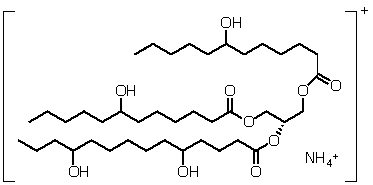
\includegraphics[height=.75in,valign=c]{images/D_TableS10_1.pdf} \\
 &  &  & MGDG 32:0 & {[}M+ NH4{]}\textsuperscript{+} & 748.5933 & -0.4 &  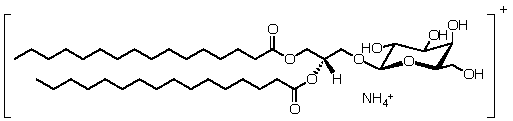
\includegraphics[height=.5in,valign=c]{images/D_TableS10_2.pdf} \\
\multirow{2}{2.5cm}[0em]{Dominant adducts of two different compounds are isobaric\emph{\textsuperscript{c}}} & C3c & 808.608 13.5 min & PE 38:0 +2O & {[}M+H{]}\textsuperscript{+} & 808.6062 & -2.3 &  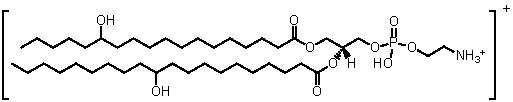
\includegraphics[height=.5in,valign=c]{images/D_TableS10_3.pdf} \\
 &  &  & DGTS 40:8 & {[}M+H{]}\textsuperscript{+} & 808.6086 & 0.7 & 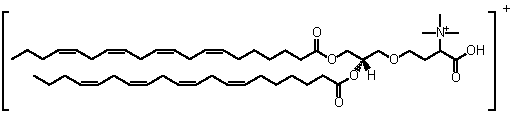
\includegraphics[height=.5in,valign=c]{images/D_TableS10_4.pdf} \\
\multirow{2}{2.5cm}[0em]{Dominant adducts of different compounds are both functional structural isomers and isobaric} & C3c, C3f & 894.6809 14.9 min & PC 40:0 +3O & {[}M+H{]}\textsuperscript{+} & 894.6794 & -1.7 &  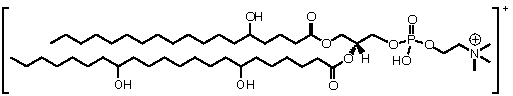
\includegraphics[height=.5in,valign=c]{images/D_TableS10_5.pdf} \\
 &  &  & PG 42:1 +1O & {[}M+NH\textsubscript{4}{]}\textsuperscript{+} & 894.6794 & -1.7 &  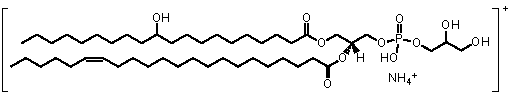
\includegraphics[height=.5in,valign=c]{images/D_TableS10_6.pdf} \\
 &  &  & TAG 52:9 +2O & {[}M+NH\textsubscript{4}{]}\textsuperscript{+} & 894.6818 & 1 &  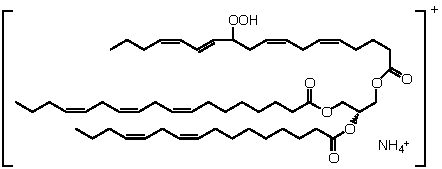
\includegraphics[height=.5in,valign=c]{images/D_TableS10_7.pdf} \\
\multirow{2}{2.5cm}[0em]{Multiple regioisomers possible for a given compound assignment\emph{\textsuperscript{d}}} & C3r & 804.5767 13.4 min, 13.1 min & PE 38:2 + 2O & {[}M+H{]}\textsuperscript{+} & 804.5749 & -2.2 & 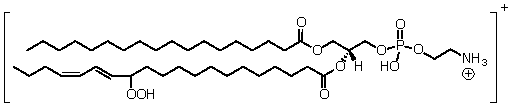
\includegraphics[height=.5in,valign=c]{images/D_TableS10_8.pdf} \\
 &  &  &  &  &  &  &  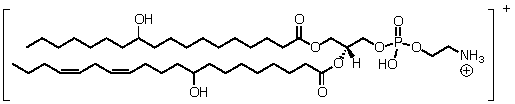
\includegraphics[height=.5in,valign=c]{images/D_TableS10_9.pdf}\\
\bottomrule
\captionsetup{font={footnotesize}}
\caption*{\emph{\textsuperscript{a}} As described in \autoref{fig:c3n1}.\\
\emph{\textsuperscript{b}} Several possible structures can be described by a given parent compound assignment; one possible structure for each assignment is shown in the table.\\
\emph{\textsuperscript{c}} In this case, the theoretical masses of the two ions were indistinguishable at the ppm (2.5) used database matching.\\
\emph{\textsuperscript{d}} Inferred from the appearance at different retention times in the same sample of multiple features with the same mass.
}
\end{longtable}
\end{flushleft}
\end{singlespace}
\end{scriptsize}

\end{landscape}

\clearpage

\begin{singlespace}
\section*{References Used in Supporting Information}
\addtocounter{section}{1}
{\setlength{\parindent}{0pt}
Clarke, K. R., P. J. Somerfield, and R. N. Gorley (2008), Testing of null hypotheses in exploratory community analyses: similarity profiles and biota-environment linkage, \emph{Journal of Experimental Marine Biology and Ecology}, 366(1-2), 56-69, \href{http://dx.doi.org/10.1016/j.jembe.2008.07.009}{doi:10.1016/j.jembe.2008.07.009}.

{\setlength{\parskip}{10pt}

Clasquin, M. F., E. Melamud, and J. D. Rabinowitz (2012), LC-MS data processing with MAVEN: a metabolomic analysis and visualization engine, \emph{Current Protocols in Bioinformatics}, 37, 14.11:14.11.11-14.11.23, \href{http://dx.doi.org/10.1002/0471250953.bi1411s37}{doi:10.1002/0471250953.bi1411s37}.

Egeland, E. S. (2011), Part VII: Data sheets aiding identification of phytoplankton carotenoids and chlorophylls, in \emph{Phytoplankton Pigments: Characterization, Chemotaxonomy and Applications in Oceanography}, edited by S. Roy, C. A. Llewellyn, E. S. Egeland and G. Johnsen, pp. 665-822, Cambridge University Press, Cambridge.

Gaquerel, E., C. Kuhl, and S. Neumann (2013), Computational annotation of plant metabolomics profiles via a novel network-assisted approach, \emph{Metabolomics}, 9(4), 904-918, \href{http://dx.doi.org/10.1007/s11306-013-0504-2}{doi:10.1007/s11306-013-0504-2}.

G\"{o}bel, C., and I. Feussner (2009), Methods for the analysis of oxylipins in plants, \emph{Phytochemistry}, 70(13-14), 1485-1503, \href{http://dx.doi.org/10.1016/j.phytochem.2009.07.040}{doi:10.1016/j.phytochem.2009.07.040}.

Kessner, D., M. Chambers, R. Burke, D. Agus, and P. Mallick (2008), ProteoWizard: open source software for rapid proteomics tools development, \emph{Bioinformatics}, 24, 2534-2536, \href{http://dx.doi.org/10.1093/bioinformatics/btn323}{doi:10.1093/bioinformatics/btn323}.

Libiseller, G., et al. (2015), IPO: a tool for automated optimization of XCMS parameters, \emph{BMC Bioinformatics}, 16, 118, \href{http://dx.doi.org/10.1186/s12859-015-0562-8}{doi:10.1186/s12859-015-0562-8}.

Melamud, E., L. Vastag, and J. D. Rabinowitz (2010), Metabolomic Analysis and Visualization Engine for LC-MS data, \emph{Analytical Chemistry}, 82(23), 9818-9826, \href{http://dx.doi.org/10.1021/ac1021166}{doi:10.1021/ac1021166}.

Patti, G. J., R. Tautenhahn, and G. Siuzdak (2012), Meta-analysis of untargeted metabolomic data from multiple profiling experiments, \emph{Nature Protocols}, 7(3), 508-516.

Popendorf, K. J., H. F. Fredricks, and B. A. S. Van Mooy (2013), Molecular ion-independent quantification of polar glycerolipid classes in marine plankton using triple quadrupole MS, \emph{Lipids}, 48(2), 185-195, \href{http://dx.doi.org/10.1007/s11745-012-3748-0}{doi:10.1007/s11745-012-3748-0}.

van den Berg, R. A., H. C. Hoefsloot, J. A. Westerhuis, A. K. Smilde, and M. J. van der Werf (2006), Centering, scaling, and transformations: improving the biological information content of metabolomics data, \emph{BMC Genomics}, 7, 142, \href{http://dx.doi.org/10.1186/1471-2164-7-142}{doi:10.1186/1471-2164-7-142}.

Warnes, G. R., et al. (2015), gplots: Various R Programming Tools for Plotting Data, R package, version 3.0.1.

Whitaker, D., and M. Christman (2014), clustsig: Significant Cluster Analysis, R package, version 1.1.

Wolf, S., S. Schmidt, M. Muller-Hannemann, and S. Neumann (2010), \emph{In silico} fragmentation for computer assisted identification of metabolite mass spectra, \emph{BMC Bioinformatics}, 11, 148, \href{http://dx.doi.org/10.1186/1471-2105-11-148}{doi:10.1186/1471-2105-11-148}.

Yang, J., K. Schmelzer, K. Georgi, and B. D. Hammock (2009), Quantitative profiling method for oxylipin metabolome by liquid chromatography electrospray ionization tandem mass spectrometry, \emph{Analytical Chemistry}, 81(19), 8085-8093, \href{http://dx.doi.org/10.1021/ac901282n}{doi:10.1021/ac901282n}.

Yang, Z.-K., Y.-F. Niu, Y.-H. Ma, J. Xue, M.-H. Zhang, W.-D. Yang, J.-S. Liu, S.-H. Lu, Y. Guan, and H.-Y. Li (2013), Molecular and cellular mechanisms of neutral lipid accumulation in diatom following nitrogen deprivation, \emph{Biotechnology for Biofuels}, 6(1), 67, \href{http://dx.doi.org/10.1186/1754-6834-6-67}{doi:10.1186/1754-6834-6-67}.}}
\end{singlespace}